\chapter{GRU应用于模拟数据本构建模研究}
% 3.2表================================================
% % 本节仅展示使用常见的三线表
% \begin{table}
%   \TableBicaption{\label{TDF_para}涵道模型参数}{Parameters of Ducted Fan Model}  % 中英文标题
%   \centering
%   \small
%   \begin{tabularx}{\textwidth}{XXXX}  % 使用 tabularx 环境,均匀分布列宽
%     \Xhline{1.5pt}
%     参数符号       & 数值                 & 参数符号  & 数值                 \tabularnewline
%     \Xhline{0.5pt}  % 表头下方线
%     $I_x$      & $054593$           & $I_y$ & $0.017045         $ \tabularnewline
%     $l_1$      & $0.0808\,\text{m}$ & $l_2$ & $0.175\,\text{m}  $ \tabularnewline
%     $l_4$      & $0.2415\,\text{m}$ & $l_5$ & $0.1085\,\text{m} $ \tabularnewline
%     $l_\sigma$ & $xdf$              & $df$  & 扫描电镜 \tabularnewline
%     \Xhline{1.5pt}
%   \end{tabularx}
% \end{table}
\section{引言}
近年来在深度学习对于流变学的本构建模中研究中,例如Lennon、Mahmoudabadbozchelou等人的研究工作,虽然细节方法各有不同,但是基本在模型选择上都选择普通多层感知机模型(MLP)\cite{lennonScientificMachineLearning2023a,mahmoudabadbozchelouDatadrivenPhysicsinformedConstitutive2021}。MLP是一种经典的前馈人工神经网络,由全连接层堆叠而成,包含输入层、多个隐藏层($\geqslant$1)及输出层,通过非线性激活函数实现复杂函数逼近。当MLP的隐藏层数到达一定值,MLP被视为深度神经网络(DNN)。传统的前馈性质的DNN模型(后简称DNN)具备一定的非线性行为捕捉能力,但是在处理时间序列数据或具有时间依赖性的数据时,其性能可能受到限制。Lennon和Mahmoudabadbozchelou的工作使用DNN模型,很难捕捉到黏弹性材料中的长程应变历史依赖性。本章的研究工作在前人的基础之上尝试使用GRU模型来构建本构建模,期待解决在处理时间序列数据时,DNN模型性能受限的问题。GRU的门控机制允许处理流变学数据,如应力应变数据时,控制历史信息的网络间流动。

本章的研究工作首先采用数值模拟方法构建了经典本构方程的应力应变模拟数据,所涉及的经典本构方程包括Herschel-Bulkley模型、Maxwell模型、Doi-Edwards模型和Giesekus模型。这些模型在流变学领域具有重要的理论和应用价值,能够描述不同类型的流变行为。首先本章研究通过数值模拟方法,生成这些模型的应力应变数据,然后对GRU模型进行了详细的构建,包括模型的结构设计、参数初始化以及训练过程中的优化策略,之后,使用数值模拟生成的应力应变数据GRU模型进行训练,通过调整模型参数和优化算法,使模型能够准确地拟合训练数据。最终本章的研究通过与DNN的训练模型对比,验证了GRU模型在处理时间序列数据时的优势。
\section{实验设计}
\subsection{数值模拟}
本章的数值模拟工作采用Python语言实现,主要依托Numpy、Scipy等高效的数值计算库来完成离散采样和数据处理。
\subsubsection{Herschel-Bulkley模型模拟}
Herschel-Bulkley模型的本构方程如公式\eqref{eq:herschel}所示,其中剪切应力$\sigma$与剪切率$\dot{\gamma}$之间存在函数关系。该模型包含流变参数$K$、流动指数$n$及屈服应力$\sigma_0$。在模拟过程中,本章设置$\sigma_0$为1.0 Pa,$K$为1,而$n$则取值为0.2、0.6、1.0、1.4及1.8。剪切率$\dot{\gamma}$范围设定为[0,100],并以0.01的时间步长进行离散采样。

数据生成后,本章首先采用Matplotlib库绘制出剪切应力$\sigma$与剪切率$\dot{\gamma}$的关系曲线,观察模拟效果,并进行生成效果评估。随后本章采用Numpy库进行数据处理,使用Pandas库将数据存储为Excel文件,便于后续的模型训练。
\subsubsection{Maxwell模型模拟}
Maxwell模型的微分本构方程如公式\eqref{eq:maxwell_model_dt}所示。该模型包含松弛时间$\tau=\eta/\\G$,其中$\eta$表示黏性系数,$G$为剪切模量。本章设置$\eta$为0.1 Pa·s,$G$为1.0 Pa。采用后向欧拉法来离散化微分方程,具体推导如下:

首先将微分离散化,设$d\sigma=\sigma_i - \sigma_{i-1}$,$dt=\Delta t$,$d\gamma=\gamma_i - \gamma_{i-1}$,则原方程可以化简为公式\eqref{eq:maxwell_euler_back_1},
\begin{equation}
  \frac{\sigma_i - \sigma_{i-1}}{\Delta t} + \frac{\sigma_i}{\tau} = G \frac{\gamma_i - \gamma_{i-1}}{\Delta t} \label{eq:maxwell_euler_back_1}
\end{equation}
移项并化简可得公式\eqref{eq:maxwell_euler_back_2}。
\begin{equation}
  \sigma_i = \frac{\sigma_{i-1} + G (\gamma_i - \gamma_{i-1})}{1 + \frac{\Delta t}{\tau}} \label{eq:maxwell_euler_back_2}
\end{equation}
根据公式\eqref{eq:maxwell_euler_back_2},本章首先使用NumPy库生成6个不同应变变化协议的应变数据,时间步为0.01,每个协议模拟2000个数据点,并存为NumPy数组,随后通过迭代法计算单个应变数据对应的应力数据,并存为NumPy数组。之后,本章使用Matplotlib库绘制出剪切应力与剪切应变的关系曲线,观察模拟效果,并进行生成效果评估。最后本章使用Pandas库将数据存储为Excel文件,便于后续的模型训练。
\subsubsection{Doi-Edwards模型模拟}
Doi-Edwards模型的本构方程如公式\eqref{eq:doi_edwards}所示。该方程为积分形式的本构方程,本章首先对该方程进行处理,将取向张量函数$\underline{Q}(t^{\prime},t)$写为球坐标形式,即公式\eqref{eq:doi_edwards_moni_q}。
\begin{align}
   & Q(t^{\prime},t) = \frac{1}{4\pi} \int_{0}^{2\pi} \int_{0}^{\pi} 5 \left( \frac{\underline{\underline{u}}^{\prime} \cdot \underline{\underline{F}}^{-1} \underline{\underline{u}}^{\prime} \cdot \underline{\underline{F}}^{-1}}{|\underline{\underline{u}}^{\prime} \cdot \underline{\underline{F}}^{-1}|^{2}} \right) \sin\theta \, d\theta \, d\phi   \label{eq:doi_edwards_moni_q} \\
   & G(t, t') = \frac{G_0}{\lambda_i} \exp\left( \frac{t' - t}{\lambda_i} \right)   \label{eq:doi_edwards_moni_g}                                                                                                                                                                                                                                                                          \\
   & \sigma(t) = \int_{t_0}^t G(t, t') \cdot Q(\gamma(t')) \, dt' \label{eq:doi_edwards_moni_sigma}
\end{align}

本章模拟的为简单剪切流动,只在xy方向存在应变,因此可以将逆变形梯度张量$\underline{\underline{F}}^{-1}$写为公式\eqref{eq:doi_edwards_f_inverse}的矩阵形式,$\underline{\underline{u}}^{\prime}$为球坐标系下的单位向量。
\begin{equation}
  \underline{\underline{F}}^{-1} = \begin{bmatrix}
    1      & 0 & 0 \\
    \gamma & 1 & 0 \\
    0      & 0 & 1
  \end{bmatrix} \label{eq:doi_edwards_f_inverse}
\end{equation}
公式\eqref{eq:doi_edwards_moni_g}为松弛模量函数,本章使用Numpy库生成7个不同的应变协议的NumPy数组,单个协议时间区间为[0,4$\pi$],总数据点为2000个,生成形式为3*3的张量矩阵,代入公式\eqref{eq:doi_edwards_moni_q}计算$Q$值数组。设置$G_0$为1.0 Pa,$\lambda$为1.0 s,$i=1$,根据公式\eqref{eq:doi_edwards_moni_sigma}计算应变张量,使用的积分工具为Python的scipy.integrate库,生成形式为3*3的张量矩阵,如公式\eqref{eq:sigma_bmatrix}所示。本章提取$
  \sigma_{12}$、$\sigma_{11}$、$\sigma_{22}$分量作为模拟实验数据,与对应的应变分量数据一起通过Pandas库存入Excel文件,便于后续的模型训练。
\begin{equation}
  \sigma = \begin{bmatrix}
    \sigma_{11} & \sigma_{12} & \sigma_{13} \\
    \sigma_{21} & \sigma_{22} & \sigma_{23} \\
    \sigma_{31} & \sigma_{32} & \sigma_{33}
  \end{bmatrix} \label{eq:sigma_bmatrix}
\end{equation}

\subsubsection{Giesekus模型模拟}
Giesekus模型的本构方程如公式\eqref{eq:giesekus}所示,迁移因子$\alpha$用于引入剪切稀化的强度。Giesekus模型模拟的为简单剪切流动,只在xy方向存在应变,应变张量$\boldsymbol{\gamma}$仅在$\gamma_{12}$分量上存在值。
本章首先使用NumPy库生成8个不同速度场协议的简单剪切流动速度数据,再使用公式\eqref{eq:giesekus-gammadot}对应生成应变速率张量数据,时间区间为[0,24],单个协议的模拟数据点为2000,生成形式为3*3应变速率张量矩阵,之后根据$\gamma_{t}=\dot{\gamma}_{t-1}\Delta t+\gamma_{t-1}$迭代计算应变张量。
\begin{equation}
  \begin{aligned}
    \dot{\gamma}_{ii} & = 2 v_{ii}(t)           \\
    \dot{\gamma}_{ij} & = v_{ij}(t) + v_{ji}(t)
  \end{aligned} \label{eq:giesekus-gammadot}
\end{equation}
随后设置迁移因子$\alpha$为0.8,其余松弛时间参数($\lambda_1$、$\lambda_2$)为1.0,使用Python的scipy.integrate.solve\_ivp函数(内置方法为Runge-Kutta法)对Giesekus模型的微分方程组进行求解计算,生成3*3应力张量矩阵,如公式\eqref{eq:sigma_bmatrix}所示。本章提取$\sigma_{12}$、$\sigma_{11}$、$\sigma_{22}$分量作为模拟实验数据,与对应的应变速率张量数据、计算后的应变张量数据一起通过Pandas库存入Excel文件,便于后续的模型训练。

\subsection{模型训练}
\subsubsection{数据集划分}
首先本章对模拟生成的数据进行数据集划分,将数据集分为训练集(Train)、验证集(Valid)和测试集(Test),不同模型的具体划分如下:

Herschel-Bulkley模型数据单独划分$n=1.0$的数据为测试集,其余数据按照9:1比例划分为训练集和验证集。

Maxwell模型单独划分4个交变应变协议为训练集和验证集,其中按照9:1比例划分为训练集和验证集。划分1个交变应变协议,1个线性应变协议为测试集。

Doi-Edwards模型单独划分5个交变应变协议为训练集和验证集,其中按照9:1比例划分为训练集和验证集。划分1个交变应变协议,1个线性应变协议为测试集。

Giesekus模型单独划分6个交变应变协议为训练集和验证集,其中按照9:1比例划分为训练集和验证集。划分1个交变应变协议,1个线性应变协议为测试集。
\subsubsection{训练细节}
本章所有模型的训练过程基本一致,首先将数据集划分后,将训练集数据和验证集数据进行归一化,之后转为Torch张量,通过Pytorch框架编写GRU模型代码进行深度学习训练。在训练过程中使用Adam优化算法,使用MSE损失函数,使用
网格搜索算法和随机搜索算法进行超参数优化和选取,训练完成将模型参数保存为.pth文件,以便后续的模型测试。

本章使用GRU和普通DNN(简单MLP)两套模型分别进行训练,训练数据集保持一致。
\subsection{模型测试}
\subsubsection{测试指标细节}
本章的模型训练均为回归问题,所以采用的测试指标为决定系数(R$^2$),如公式\eqref{eq:r2},平均绝对误差(MAE),如公式\eqref{eq:mae}和平均百分比误差(MAPE),如公式\eqref{eq:mape}。
\begin{equation}
  \text{R}^2 = 1 - \frac{\sum_{i=1}^{n} (y_i - \hat{y}_i)^2}{\sum_{i=1}^{n} (y_i - \bar{y})^2} \label{eq:r2}
\end{equation}
\begin{equation}
  \text{MAE} = \frac{1}{n} \sum_{i=1}^{n} |y_i - \hat{y}_i| \label{eq:mae}
\end{equation}
\begin{equation}
  \text{MAPE} = \frac{100\%}{n} \sum_{i=1}^{n} \left| \frac{y_i - \hat{y}_i}{y_i} \right| \label{eq:mape}
\end{equation}
此外,加上训练时间(Training Time)作为训练成本指标。
\subsubsection{不同模型的测试实验划分}
Herschel-Bulkley模型使用训练后保存的模型参数,使用测试集时间进行预测,训练数据与测试数据为不同的流动指数$n$,采用已知流动指数数据预测未知流动指数数据,预测物理量为剪切应力(Stress)。按照上述实验步骤分别使用DNN和GRU两种模型进行测试,绘制两个模型的测试比对曲线。

Maxwell模型训练数据为交变应变数据,其应变关系符合公式\eqref{eq:sin_gamma_protocol},测试数据分为交变应变数据和线性应变数据(公式\eqref{eq:linear_gamma_protocol})。采用已知交变协议数据预测未知交变协议数据,已知交变协议数据预测未知线性协议数据,预测物理量为剪切应力(Stress)。按照上述实验步骤分别使用DNN和GRU两种模型进行测试,绘制两个模型的测试比对曲线。对于GRU模型,设置不同的序列时间步进行训练,探究模型的最佳时间步。
\begin{equation}
  \gamma=\gamma_0cos(\omega t+\phi) \label{eq:sin_gamma_protocol}
\end{equation}
\begin{equation}
  \gamma=\dot{\gamma}t \label{eq:linear_gamma_protocol}
\end{equation}

Doi-Edwards模型和Giesekus模型与Maxwell模型的实验流程一致,采用已知交变协议数据预测未知交变协议数据,已知交变协议数据预测未知线性协议数据,预测物理量为xy方向剪切应力($\sigma_{12}$)和第一法向应力差($\text{N}_1$)。第一法向应力差的公式为$\text{N}_1=\sigma_{11}-\sigma_{12} $,表示模拟流体的弹性行为。按照上述实验步骤分别使用DNN和GRU两种模型进行测试,绘制两个模型的测试比对曲线。对于GRU模型,设置不同的序列时间步进行训练,探究模型的最佳时间步。
\section{结果与讨论}
\subsection{Herschel-Bulkley模型建模}
\subsubsection{数值模拟数据}
本节使用Herschel-Bulkley模型模拟数据,模拟结果如图\ref{herschel_moni}所示。由图\ref{herschel_moni}可以看到,模拟数据中剪切应力(Stress)与剪切速率(Shear Rate)呈现幂函数关系,随着流变指数$n$的增加,曲线的斜率增大,表明流体的非牛顿特性增强。这一现象与Herschel-Bulkley模型的数学形式相符,说明模拟数据符合预期。
\begin{figure}[htbp]
  \centering
  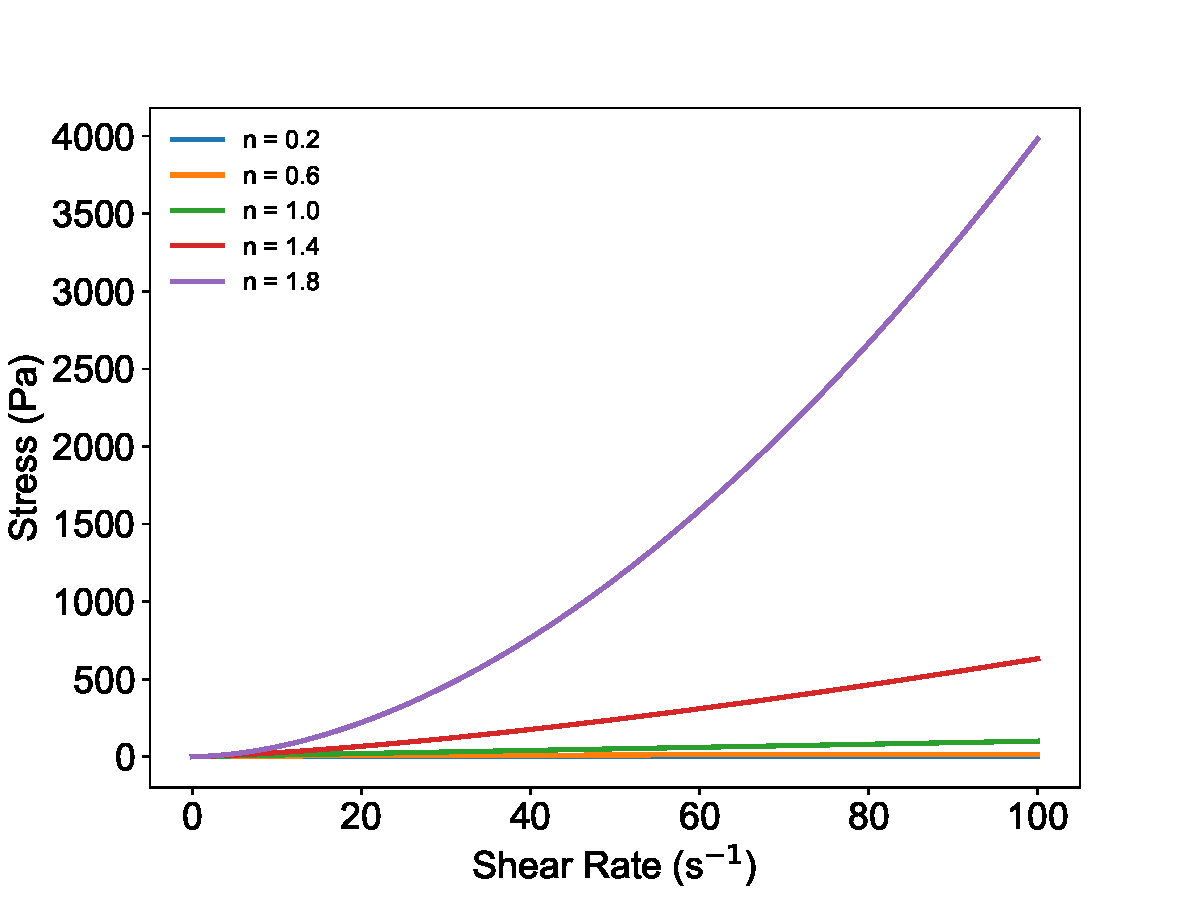
\includegraphics[width=0.8\textwidth]{Fig/herschel_moni.pdf}
  \FigureBicaption{\label{herschel_moni}Herschel-Bulkley模型模拟数据应力-应变率曲线图,n为流变指数}{Stress–strain rate curve of simulated data for the Herschel-Bulkley model, where n represents the flow index}
\end{figure}
\subsubsection{GRU/DNN模型预测效果对比}
本节分别使用GRU和DNN两种算法对Herschel-Bulkley模型模拟数据进行深度学习建模,之后使用预测模型在测试集上进行验证,测试结果如图\ref{herschel_test}所示。图\ref{herschel_test}(a)为两种算法测试的真实值-预测值曲线,从曲线可以定性看出两种算法的预测值曲线与真实值曲线都非常接近。图\ref{herschel_test}(b)为两种算法测试结果的残差图,可以看出两种算法的残差点离散程度接近,均没有明显趋向性,均呈现无序分布,说明两种算法均可以比较好地捕捉到所有的输入特征。图\ref{herschel_test}(c-f)分别比较了两种算法预测结果的R$^2$,MAE,MAPE指标,从结果中可以看出,两种算法的预测效果都十分良好,R$^2$都接近1,GRU预测结果的R$^2$值略高于DNN,GRU预测结果的MAE和MAPE值都小于DNN,但数值差距不大。GRU算法的平均训练时间为378 s,高于DNN的155 s 一倍以上,这是由于GRU网络的参数量更大,且由于其循环神经网络的特点,只能顺序运算,限制了GPU的并行计算能力,导致训练时间较长。

综合看来GRU和DNN两种算法在Herschel-Bulkley模型模拟数据上的预测表现比较接近,从预测指标的绝对数值看,GRU略优于DNN。这个结果符合预期,因为Herschel-Bulkley模型本质上是模拟了剪切稀化增稠过程,不涉及黏弹性材料的时间依赖性,并且我们模拟的过程中,对于某个特定时间的应力状态也仅仅是当前应变状态的函数。从训练时间的分析看,GRU的训练成本远高于DNN。综合而言对于本构方程类似于Herschel-Bulkley模型的流体,GRU算法虽然在泛化效果上略有优势,但是综合性能上不具备显著优势。
\begin{figure}[htbp]
  \centering
  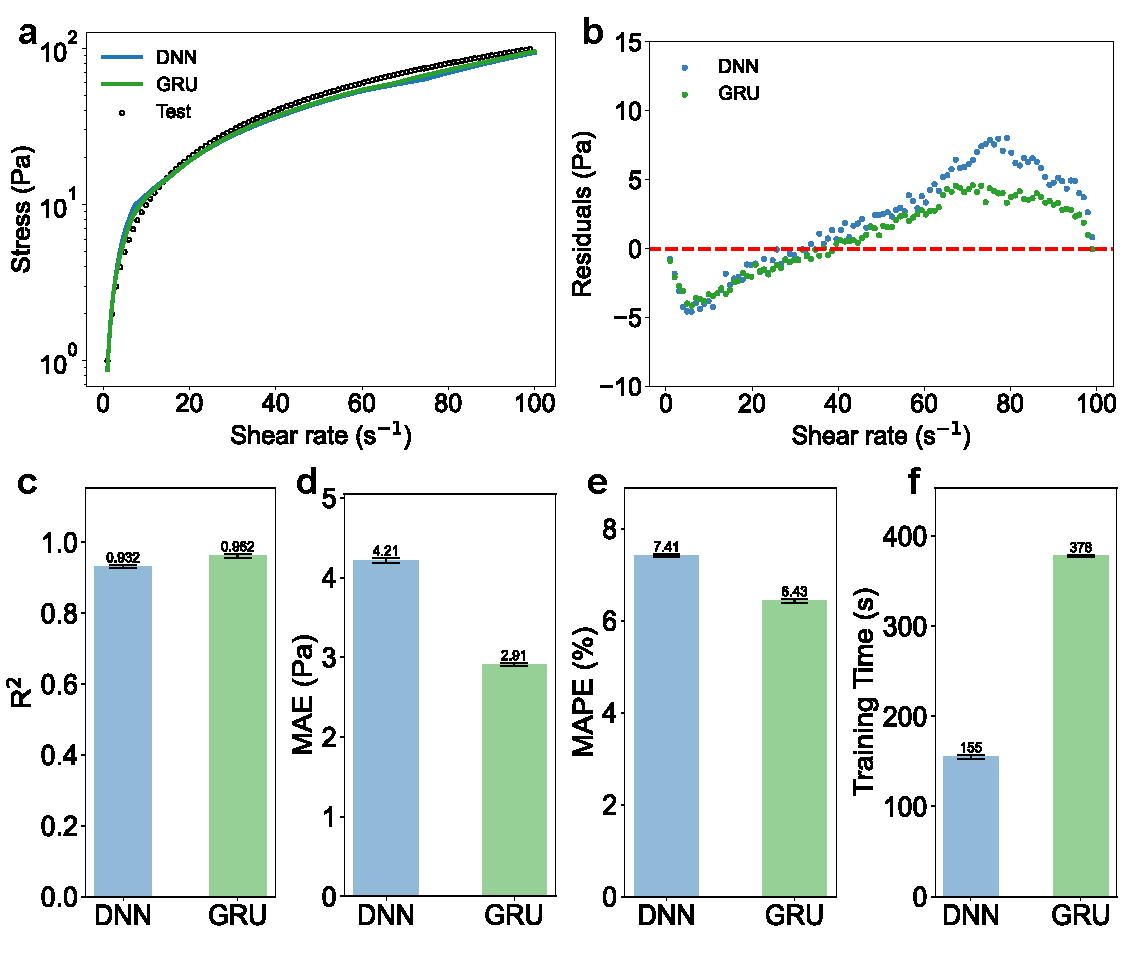
\includegraphics[width=0.8\textwidth]{Fig/Herschel_test.pdf}
  \FigureBicaption{\label{herschel_test}GRU算法和DNN算法在Herschel-Bulkley模型测试集上的预测效果对比示意图:(a)GRU和DNN在训练建模后的预测值-真实值曲线图;(b)GRU和DNN训练建模后的预测值残差图;(c)GRU和DNN测试集上的R$^2$指标图;(d)GRU和DNN在测试集上的MAE指标图;(e)GRU和DNN在测试集上的MAPE指标图;(f)GRU和DNN在测试集上的训练时间指标图}{Comparison schematic of the prediction performance of the GRU algorithm and the DNN algorithm on the Herschel-Bulkley model test set: (a) Predicted value–true value curves for GRU and DNN after training and modeling; (b) Residual plots of the predicted values for GRU and DNN after training and modeling; (c) R$^2$ metric plots on the test set for GRU and DNN; (d) MAE metric plots on the test set for GRU and DNN; (e) MAPE metric plots on the test set for GRU and DNN; (f) Training Time metric plots on the test set for GRU and DNN}
\end{figure}
\subsection{Maxwell模型建模}
\subsubsection{数值模拟数据}
本节通过后向欧拉法对简单 Maxwell 模型进行了数值模拟,生成了模拟数据,并绘制了应力-应变曲线(Lissajous 曲线),结果如图 \ref{maxwell_moni} 所示。图 \ref{maxwell_moni} 展示了不同应变协议下的模拟结果。对于正弦交变应变,Lissajous 曲线呈现出标准的闭合椭圆形状,这与 Maxwell 模型的理论预期一致,表明模型在周期性应变下的响应具有良好的稳定性和可预测性。对于线性应变,Lissajous 曲线在应变较小时表现出应力的快速增加,随后随着应变的继续增加,应力逐渐趋于一个稳定值,这一现象同样符合 Maxwell 模型的理论预期,反映了材料在持续应变下的应力松弛特性。综合看来,后向欧拉法模拟的数据符合预期,可以用于后续训练。
\begin{figure}[htbp]
  \centering
  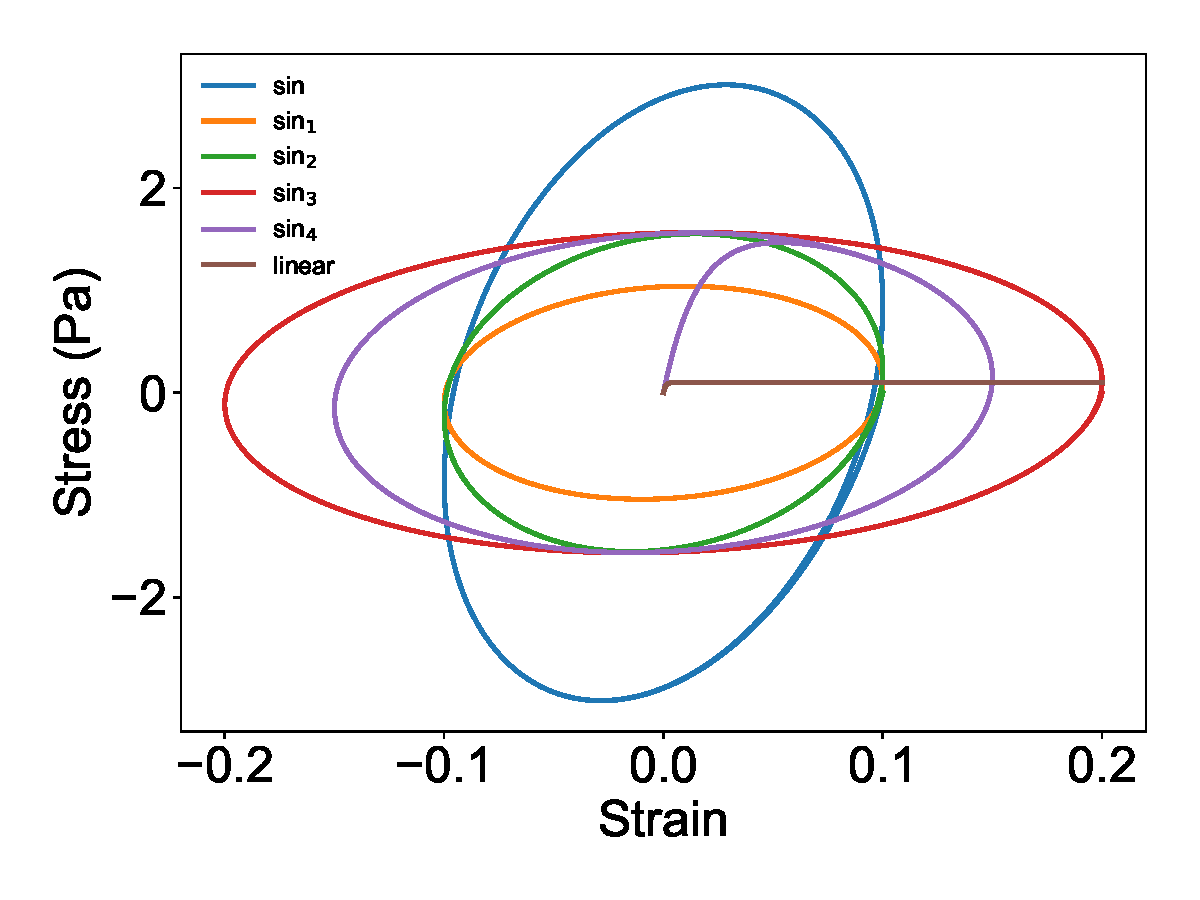
\includegraphics[width=0.8\textwidth]{Fig/maxwell_moni.pdf}
  \FigureBicaption{\label{maxwell_moni}不同应变变化协议的Maxwell模型模拟数据应力-应变曲线(Lissajous曲线)图}{Stress–strain curves (Lissajous curves) of simulated data for the Maxwell model under different strain variation protocols}
\end{figure}

\subsubsection{交变协议预测交变协议效果验证}
为了验证GRU算法在时间序列本构方程数据中的预测效果,本节使用交变应变协议生成的数据作为训练集,交变应变协议生成的数据作为测试集。分别使用了GRU和DNN进行训练,并在测试集上进行验证,测试结果如图\ref{maxwell_sin}、图\ref{maxwell_sin_metric}所示。

图\ref{maxwell_sin}(a-b)为两种不同算法预测模型在测试集上的真实值-预测值曲线,
图a为Lissajous曲线,可以看到GRU算法的预测值的Lissajous曲线与真实值曲线十分接近,而DNN算法的预测值的Lissajous曲线与真实的曲线则有明显的周期性偏差,尤其在大应变时,预测值与真实值有较大的偏差。图b为时间-应力曲线,从中可以看到GRU算法的预测值曲线随时间变化较为稳定,贴近真实值曲线,而DNN算法的预测值的曲线明显偏离真实值曲线。

图\ref{maxwell_sin}(c)为两种算法预测模型的测试集残差图,从图中可以看到DNN算法的预测值与真实值残差呈现非常明显的周期性分布,说明DNN未能捕捉到训练数据中的周期性特征,或者说无法泛化到测试集。而GRU的残差图则为无序的近似正态分布,虽然局部存在一定周期性,但是总体正态分布效果明显由于DNN的对应残差,这说明GRU捕捉到了训练数据的较完整的特征,尤其是DNN未能捕捉的周期性特征。综合真实值-预测值曲线和残差图,可以定性分析出GRU的预测效果更为优秀。
\begin{figure}[htbp]
  \centering
  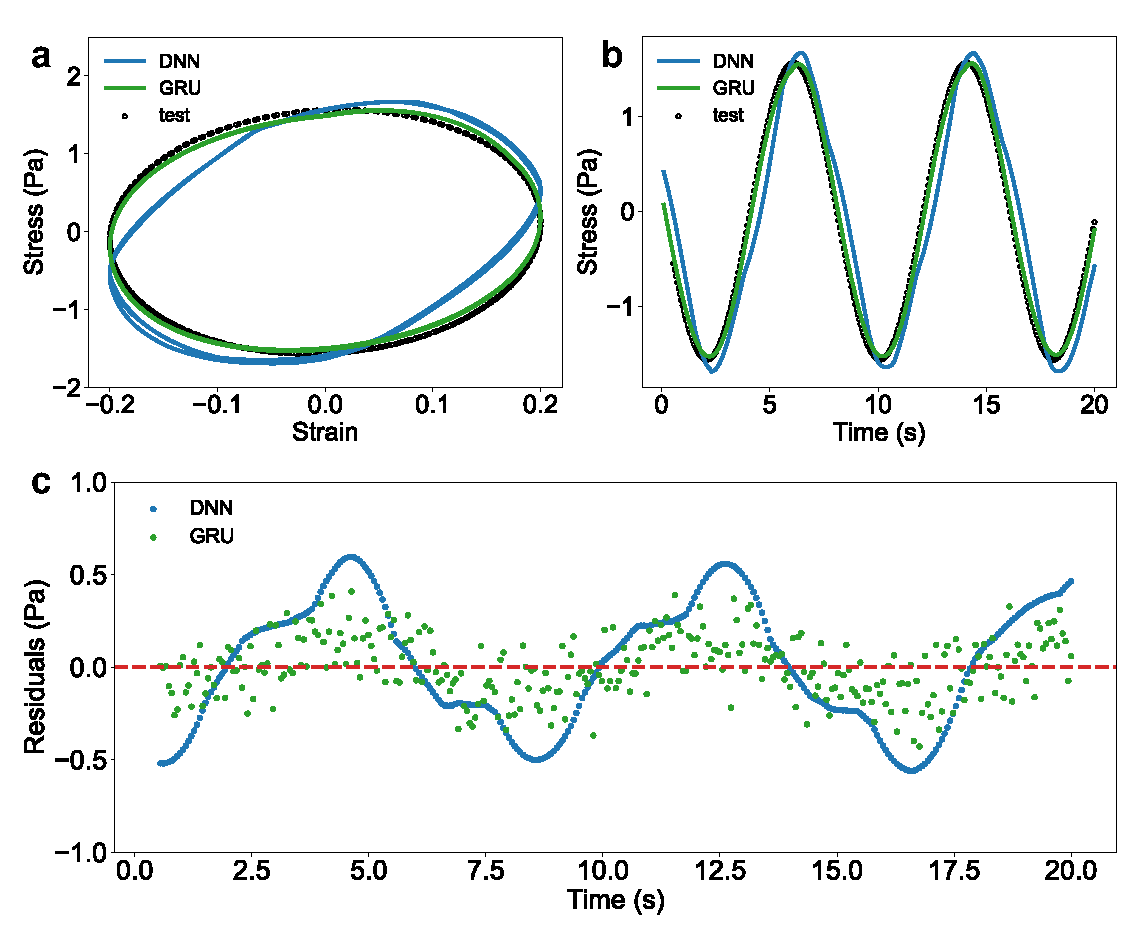
\includegraphics[width=0.8\textwidth]{Fig/Maxwell_sin_.pdf}
  \FigureBicaption{\label{maxwell_sin}GRU算法和DNN算法在Maxwell模型测试集上的预测效果对比示意图:(a)GRU和DNN在测试集上的预测值与真实值的应力-应变曲线(Lissajous曲线);(b)GRU和DNN在测试集上的预测值与真实值的应力-时间曲线;(c)GRU和DNN在测试集上的预测值残差图}{Comparison schematic of the prediction performance of the GRU algorithm and the DNN algorithm on the Maxwell model test set: (a) Stress–Strain curves (Lissajous curves) of predicted and true values for GRU and DNN on the test set; (b) Stress–Time curves of predicted and true values for GRU and DNN on the test set; (c) Residual plots of predicted values for GRU and DNN on the test set}
\end{figure}
接下来,本节计算两种算法的测试集预测指标,绘制指标对比图\ref{maxwell_sin_metric}。从图\ref{maxwell_sin_metric
}(a)显示,GRU的R$^2$值为0.986,接近1,说明GRU的预测效果十分优秀,而DNN的R$^2$值为0.904,略低于GRU,但是也高于0.9,属于非常出色的指标。仅从R$^2$指标来看,GRU预测效果优于DNN,但是优势不明显。从图\ref{maxwell_sin_metric}(b-c)看,GRU预测结果的MAE值为0.019,仅为DNN预测结果的MAE值的一半,GRU预测结果的MAPE值为1.89,仅为DNN预测结果的MAPE值3.35的一半。这定量说明GRU的预测结果误差远小于DNN的预测结果误差,GRU在此项任务上预测泛化效果更好。当然,由于GRU的模型特性,其训练时间如图\ref{maxwell_sin_metric}(d)所示,要高于DNN。
\begin{figure}[htbp]
  \centering
  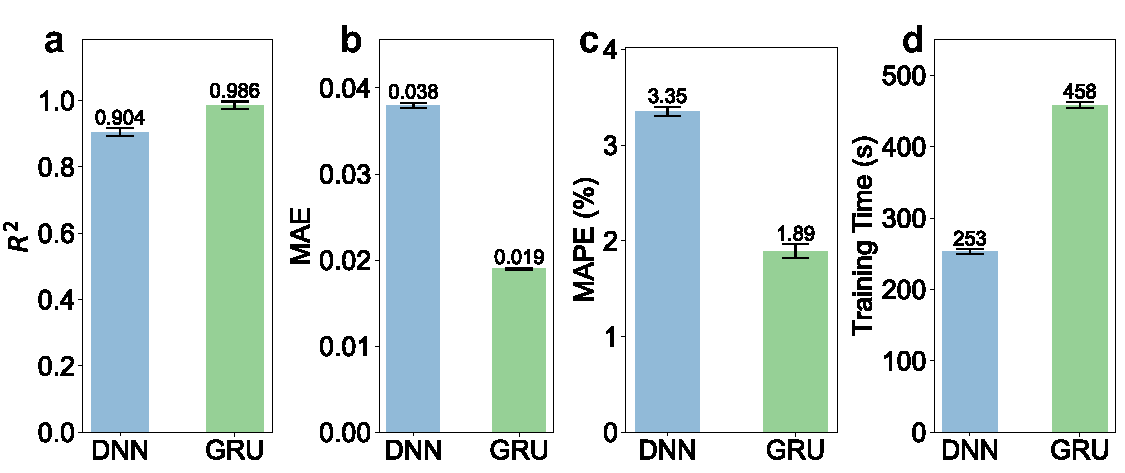
\includegraphics[width=0.8\textwidth]{Fig/Maxwell_sin_metric.pdf}
  \FigureBicaption{\label{maxwell_sin_metric}}{}
\end{figure}
综合各项分析数据来看,当训练数据和测试数据为同类型应变变化过程(都为交变应变)时,GRU算法可以更好的学习到Maxwell模型数据的内在特征,包括周期性响应,黏弹性,时间依赖性响应。从定性与定量分析结果看,GRU算法的预测泛化效果在此项任务上明显优于DNN,在计算资源足够时,GRU算法相比DNN性能更佳。


\subsubsection{交变协议预测线性协议效果验证}
为了验证GRU算法在不同形式的应变历史下的泛化预测效果,本节使用交变应变协议生成的数据作为训练集,线性应变协议生成的数据作为测试集。分别使用了GRU和DNN进行训练,并在测试集上进行验证,测试结果如图\ref{maxwell_linear}、图\ref{maxwell_linear_metric}所示。

图\ref{maxwell_linear}(a)为两种不同算法预测模型在测试集上的真实值-预测值的Lissajous曲线,图中可以看到GRU算法的预测值的Lissajous曲线与真实值曲线接近,在小应变时有一定偏差,这可能源于门控单元对初始状态记忆单元的权重初始化敏感性问题。而DNN算法的预测值的Lissajous曲线与真实的曲线相比GRU偏差更大,在小应变时,预测值与真实值有较大的偏差。

图\ref{maxwell_linear}(b)为两种算法预测模型的测试集残差图,从图中可以看到DNN算法的预测值与真实值残差分布不均匀,在小应变时为单调增曲线趋势,在Strain=0.25处存在明显峰,整体呈现清晰曲线趋势,说明DNN未能捕捉到训练数据中的关键特征,在测试集上表现较差。而GRU的残差图则为无序分布,总体分布效果明显优于DNN的对应残差,GRU的残差图残差点均匀分布在0刻度线两侧,残差值相比DNN较小。这说明GRU捕捉到了训练数据的较完整的特征,且预测偏差较小。综合真实值-预测值曲线和残差图,可以定性分析出GRU的预测效果更为优秀。
\begin{figure}[htbp]
  \centering
  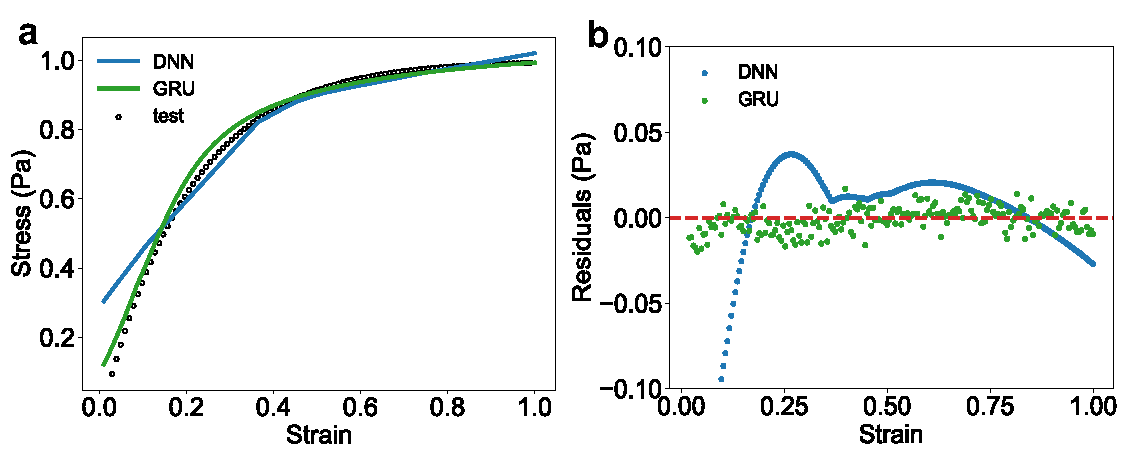
\includegraphics[width=0.8\textwidth]{Fig/maxwell_linear_test.pdf}
  \FigureBicaption{\label{maxwell_linear}}{}
\end{figure}
接下来,本节计算两种算法的测试集预测指标,绘制指标对比图\ref{maxwell_linear_metric}。图\ref{maxwell_linear_metric}(a)显示,GRU的R$^2$值为0.976,接近1,证明GRU的预测效果十分优秀,而DNN的R$^2$值为0.908,略低于GRU,但是也高于0.9,属于非常出色的指标。仅从R$^2$指标来看,GRU预测效果优于DNN,但是优势不明显。从图\ref{maxwell_linear_metric}(b-c)看,GRU预测结果的MAE值为0.071,而DNN的预测结果的MAE值为0.293,GRU在绝对误差上仅为DNN的四分之一,优势显著。GRU预测结果的MAPE值为3.09,仅为DNN预测结果的MAPE值14.95的五分之一左右。这定量说明GRU的预测结果误差远小于DNN的预测结果误差,GRU在此项任务上预测泛化效果更好。这里的训练时间对比与上一节的交变协议预测交变协议一致,同图\ref{maxwell_sin_metric}(d)所示。
\begin{figure}[htbp]
  \centering
  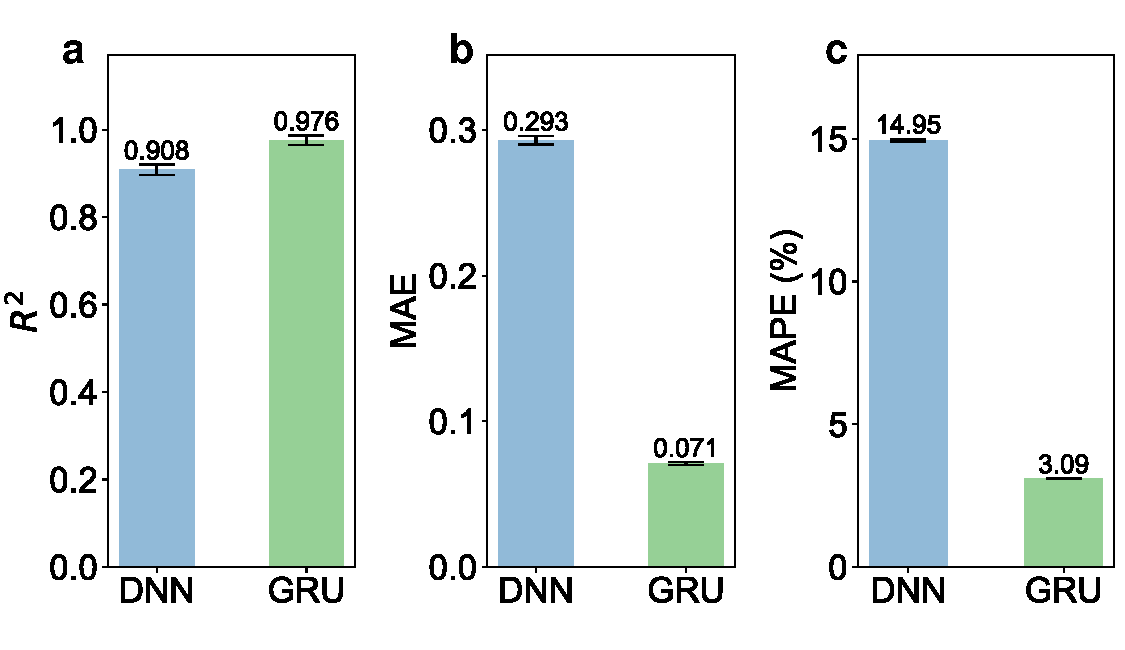
\includegraphics[width=0.8\textwidth]{Fig/maxwell_linear_metric.pdf}
  \FigureBicaption{\label{maxwell_linear_metric}}{}
\end{figure}

综合各项分析数据来看,当训练数据和测试数据为不同类型应变变化过程时,GRU算法展现出了显著的优势,尤其是在学习Maxwell模型数据的内在特征方面。Maxwell模型作为一种经典的粘弹性模型,其核心在于描述材料在应力作用下的时间依赖性响应。GRU算法可以仅通过学习交变应变的训练数据,就能够很好地预测线性应变的测试数据。这是因为GRU算法能够有效地从交变应变数据中提取出关键的时间依赖性特征,并将其应用于线性应变的预测中。
\subsubsection{不同时间步的预测效果对比}
对于GRU这类循环神经网络来说,网络架构的时间步数(序列长度)是非常重要的超参数。较大的时间步可以使模型在每个时间步上处理更多的信息,有助于捕捉长期依赖关系,但是可能导致模型学习到数据中的噪声,而不是其潜在的结构,从而导致过拟合。较小的时间步较小的时间步可以更细致地捕捉序列中的短期变化和细节信息,有助于模型更好地理解数据的短期动态特征,可能导致模型过于关注噪声,而忽略重要的长期依赖关系,从而导致欠拟合。本节研究了不同时间步下训练的模型在测试集上的预测效果。如图\ref{maxwell_timesteps_metrics}所示。由图可见,预测模型R$^2$值随着时间步的增加而增加,但是幅度较小。MAE值和MAPE值随时间步的增加而减少,说明随着时间步的增加,模型的预测效果变的更好,时间步小于10时,这种误差减小的趋势较明显,时间步大于20时,MAE值下降幅度变小,时间步大于10,MAPE值下降幅度变小。这说明模型的优化指标上升存在阈值,这是因为GRU算法在较长序列中容易遗忘丢失信息,对于时间序列的处理长度有一定限制。而随着时间步的增加,当时间步大于20后,模型的训练时间急剧增加,训练成本陡增。

本节分析针对此项任务,最佳时间步在10-20之间,MAE值和MAPE值开始下降到阈值,且训练时间还未显著增加。
\begin{figure}[htbp]
  \centering
  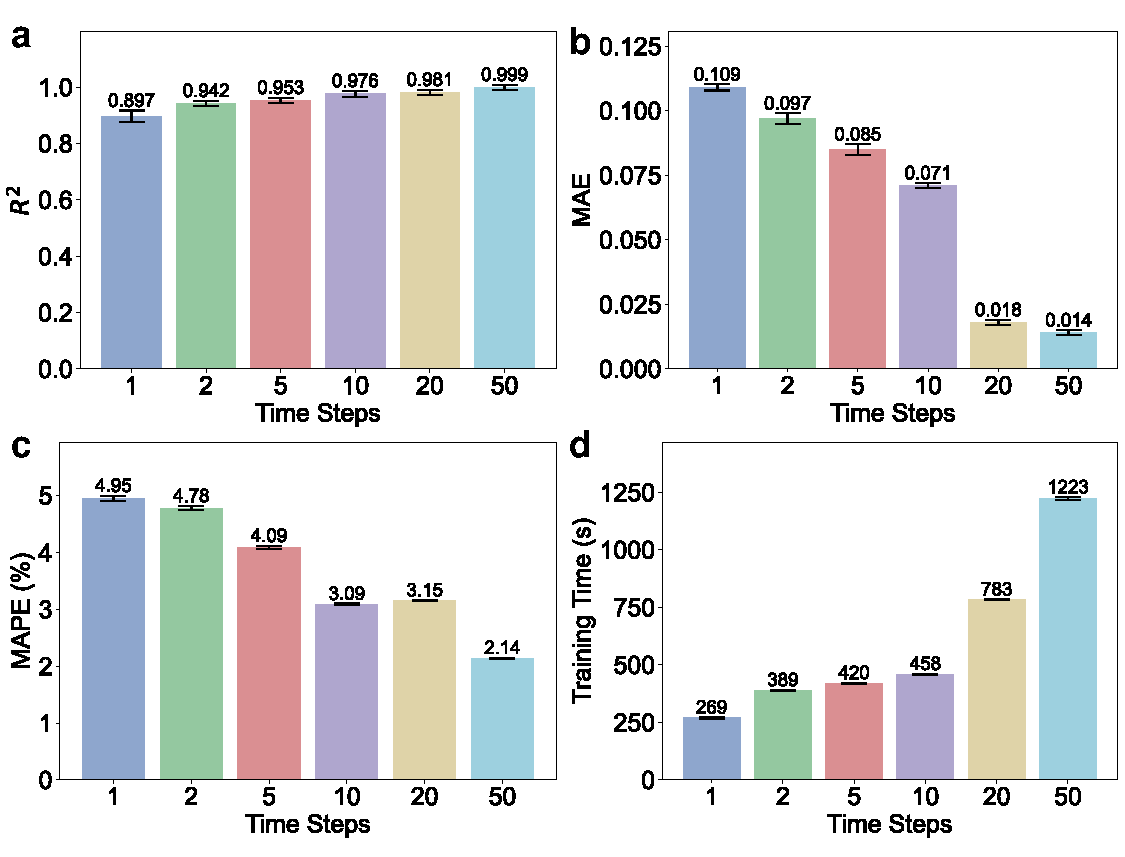
\includegraphics[width=0.8\textwidth]{Fig/Maxwell_timesteps_metrics.pdf}
  \FigureBicaption{\label{maxwell_timesteps_metrics}}{}
\end{figure}

% Doi-Edwards模型建模
\subsection{Doi-Edwards模型建模}
\subsubsection{数值模拟数据}
本节使用Python的scipy.integrate库对Doi-Edwards模型进行数值积分模拟。模拟结果如图\ref{doi-edwards-moni}所示。图\ref{doi-edwards-moni}(a)为不同应变振幅模拟的剪切应力应变Lissajous曲线,曲线呈现标准的椭圆形状,符合Doi-Edwards模型在小应变下的假设。图\ref{doi-edwards-moni}(b)为模拟的第一法向应力差(N$_1$)的Lissajous曲线,曲线具有振幅依赖性,且为滞回曲线,与文献中的Doi-Edwards模型一致。图\ref{doi-edwards-moni}(c)为线性应变协议下的应力-时间曲线,可以看到随着应变加载,应力一开始为近似的线性增加,后逐渐趋向平台值,这个结果符合预期。综上本节模拟的数据可以认为符合Doi-Edwards模型,可以用于后续实验。
\begin{figure}[htbp]
  \centering
  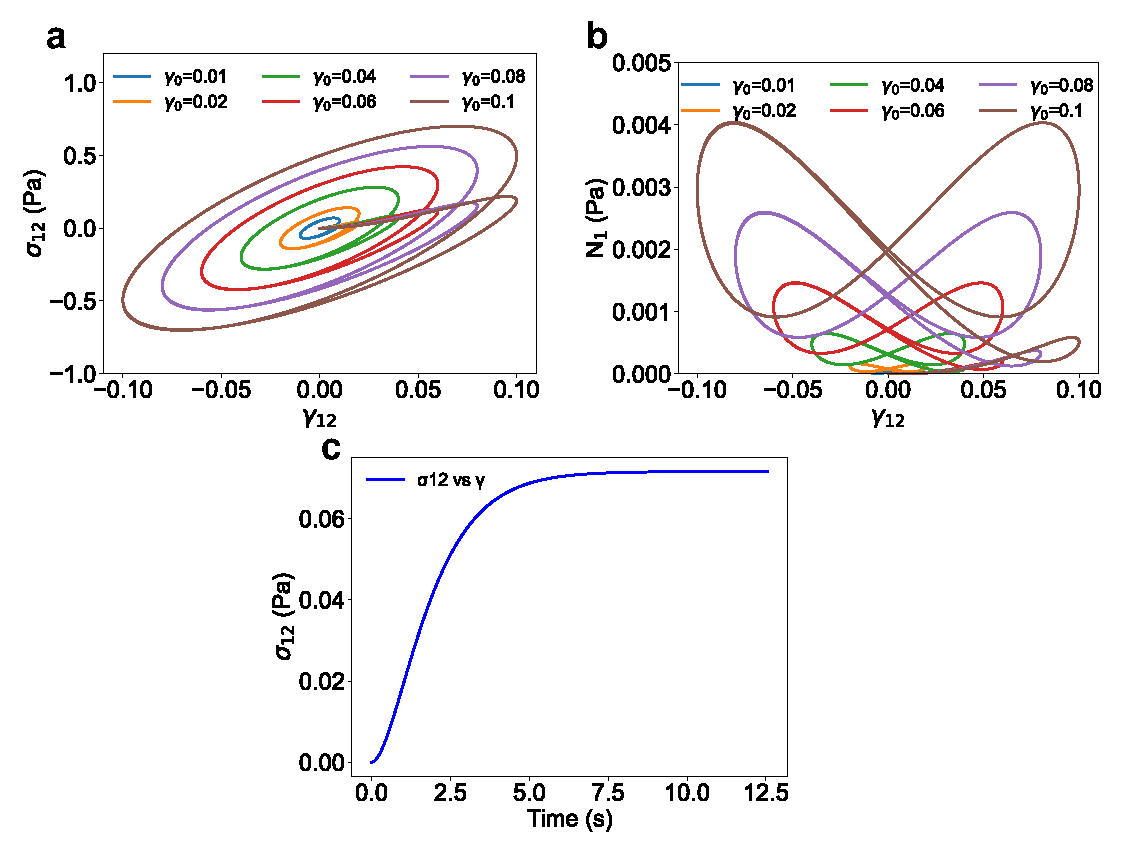
\includegraphics[width=0.8\textwidth]{Fig/doi-edwards-moni.pdf}
  \FigureBicaption{\label{doi-edwards-moni}}{}
\end{figure}
\subsubsection{交变协议预测交变协议效果验证}
为了验证GRU算法在Doi-Edwards模型本构方程数据中的预测效果,本节使用交变应变协议生成的数据作为训练集,交变应变协议生成的数据作为测试集。分别使用了GRU和DNN进行训练,并在测试集上进行验证,测试结果如图\ref{doi-edwards-sin}、图\ref{doi-edwards-sin-metric}所示。

图\ref{doi-edwards-sin}(a-c)为两种不同算法构建的预测模型预测的剪切应力($\sigma_{12}$)的Lissajous曲线、时间-应力曲线、残差图,(d-f)为预测的第一法向应力差(N$_{1}$)的Lissajous曲线、时间-应力曲线、残差图。
图a和图b可以看出GRU算法的预测的$\sigma_{12}$值与真实的$\sigma_{12}$接近,曲线拟合较好。而DNN算法的预测值在某些区域存在较大误差,例如在应变变化的初始和5-10 s之间,DNN存在较大误差。图c的残差图则显示,GRU算法预测值与真实值的残差紧贴0刻度线,呈现无序离散的分布状态,而DNN算法预测值和真实值的残差呈现明显的曲线规律,且与0刻度线性距离偏差较大,残差分布区间远远大于GRU部分。残差图的结果表明对于GRU成功地学习到了训练数据中的各项特征,复杂的非线性关系,且不存在明显周期性,总体残差较小,而DNN存在特征未能完全学习的问题,拟合效果较差,未能很好地捕捉到训练数据的特征。从图d、图e和图f的N$_1$的预测效果图来看,N$_1$与$\sigma_{12}$的结果类似,均是GRU的预测效果要由于DNN,而对比GRU预测的N$_1$值和$\sigma_{12}$值,则是$\sigma_{12}$值的预测效果会更好,这可能是因为$\sigma_{12}$与输入的剪切速率特征$\dot{\gamma_{12}}$之间的函数关系更为简单,且更加符合时间叠加原理,所以GRU可以更好地捕捉其时间依赖性和内在联系。
\begin{figure}[htbp]
  \centering
  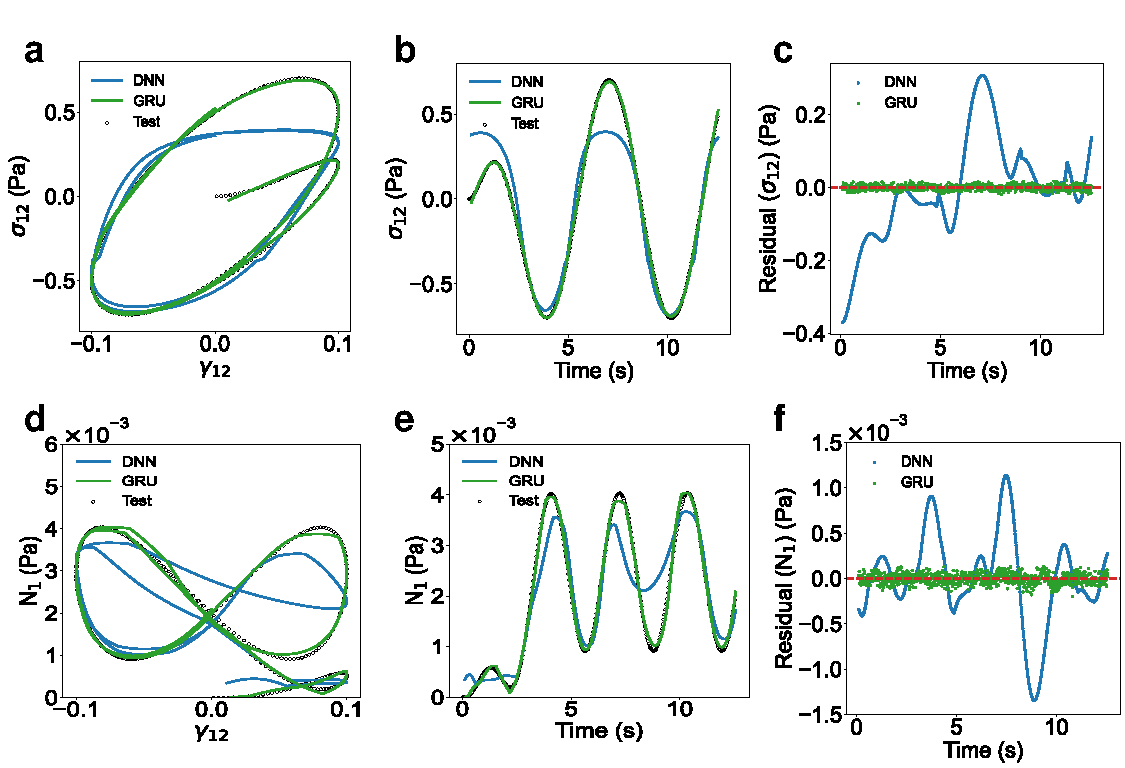
\includegraphics[width=0.8\textwidth]{Fig/doi-edwards-sin.pdf}
  \FigureBicaption{\label{doi-edwards-sin}}{}
\end{figure}

之后本节分别对两种不同算法在$\sigma_{12}$和N$_1$上的预测效果做了定量分析,指标图如图\ref{doi-edwards-sin-metric}所示。在R$^2$指标上,GRU在$\sigma_{12}$和N$_1$的预测指标均优于DNN,而同种算法下$\sigma_{12}$的R$^2$值要高于N$_1$,显示$\sigma_{12}$的预测效果更好。在MAE指标上,DNN的$\sigma_{12}$和N$_1$的MAE值均远高于GRU,说明GRU的预测误差远小于DNN。MAPE指标与MAE指标的对比基本一致,都是GRU的预测误差小于DNN。但是同种算法下$\sigma_{12}$的MAE值高于N$_1$,但是MAPE值反之,这是因为MAE值强调的是绝对值比较,受到真实数据本身尺度的影响,因此比较同种算法下$\sigma_{12}$和N$_1$的预测效果应当以去除了数据尺度影响的MAPE值来判定,而MAPE值的结论表明同种算法下$\sigma_{12}$值的预测效果相比N$_1$更好,这与R$^2$的分析和图\ref{doi-edwards-sin}的定性分析一致,这也是后续可以优化的方向之一。最后,从图\ref{doi-edwards-sin-metric}(d)来看,GRU在此项任务上的训练时间为DNN的3倍左右,符合更高成本的预期。
\begin{figure}[htbp]
  \centering
  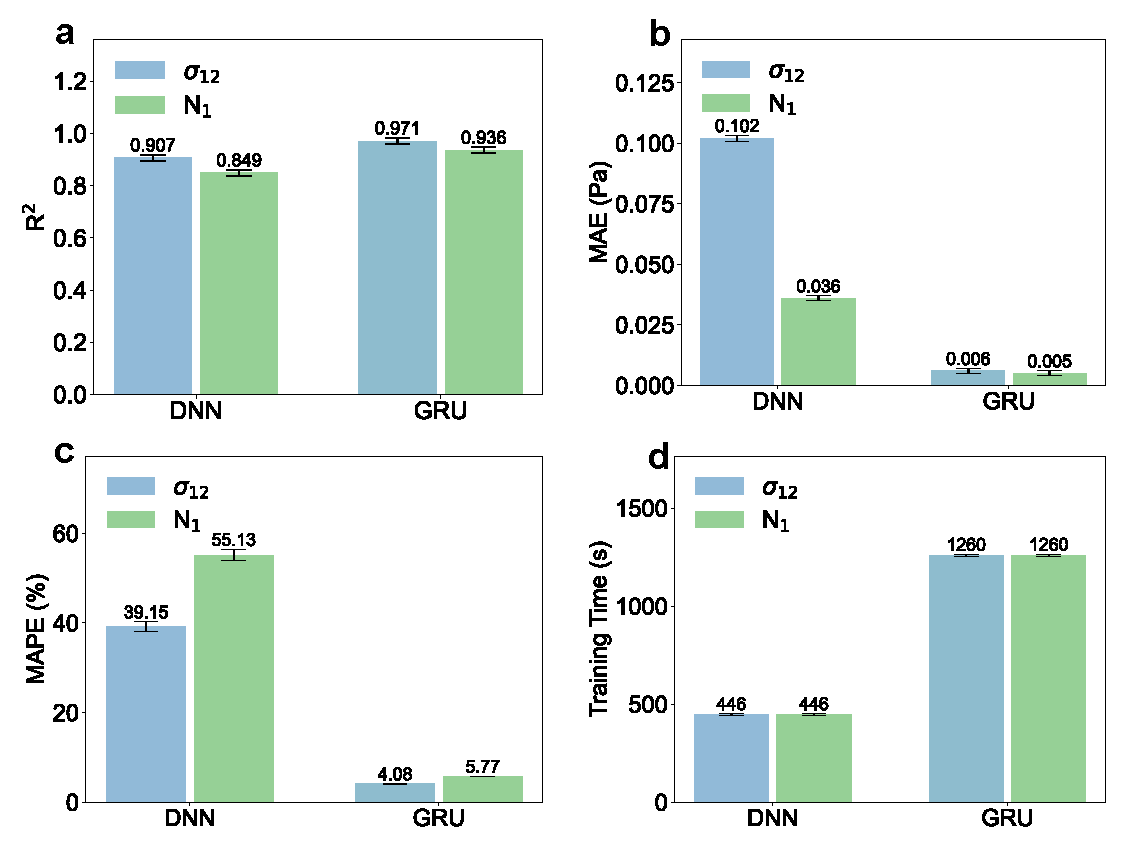
\includegraphics[width=0.8\textwidth]{Fig/doi-edwards-sin-metrics.pdf}
  \FigureBicaption{\label{doi-edwards-sin-metric}}{}
\end{figure}
综合各项分析数据来看,当训练数据和测试数据为同类型应变变化过程(都为交变应变)时,GRU算法可以更好的学习到Doi-Edwards模型数据的内在特征,包括周期性响应,黏弹性,时间依赖性响应。从定性与定量分析结果看,GRU算法的预测泛化效果在此项任务上明显优于DNN,在计算资源足够时,GRU算法相比DNN性能更佳,而在同种算法下$\sigma_{12}$的预测效果优于N$_1$。
\subsubsection{交变协议预测线性协议效果验证}
为了验证GRU算法在不同形式的应变历史下对于Doi-Edwards模型泛化预测效果,本节使用交变应变协议生成的数据作为训练集,线性应变协议生成的数据作为测试集。分别使用了GRU和DNN进行训练,并在测试集上进行验证,测试结果如图\ref{doi-edwards-linear}、图\ref{doi-edwards-linear-metrics}所示。

图\ref{doi-edwards-linear}(a)为两种不同算法预测模型在测试集上的真实值-预测值曲线,图中可以看到GRU算法的预测值的曲线与真实值曲线接近,无较明显的偏差区间,而DNN算法的预测值的曲线与真实的曲线存在明显的偏差。在应变加载初始和结束时,DNN算法的预测值相比真实值偏大,而应变加载2-6 s的中间阶段,DNN算法的预测值又偏小,总体来看仅在大致趋势上符合真实值曲线。

图\ref{doi-edwards-linear}(b)展示了两种算法在测试集上的残差图。从图中可以明显看出,DNN算法的预测值与真实值之间的残差分布并不均匀,整体呈现出较为清晰的曲线趋势,尤其是在3秒附近出现了显著的峰值。这表明DNN未能充分捕捉到训练数据中的关键特征,导致其在测试集上的表现不尽如人意。相比之下,GRU算法的残差图则呈现出无序分布,残差点均匀地分布在0刻度线两侧,且残差值普遍小于DNN。这说明GRU能够更好地捕捉到训练数据中的特征,预测偏差也更小。综合真实值与预测值的曲线以及残差图的分析,可以定性地得出结论:GRU的预测效果优于DNN。
\begin{figure}[htbp]
  \centering
  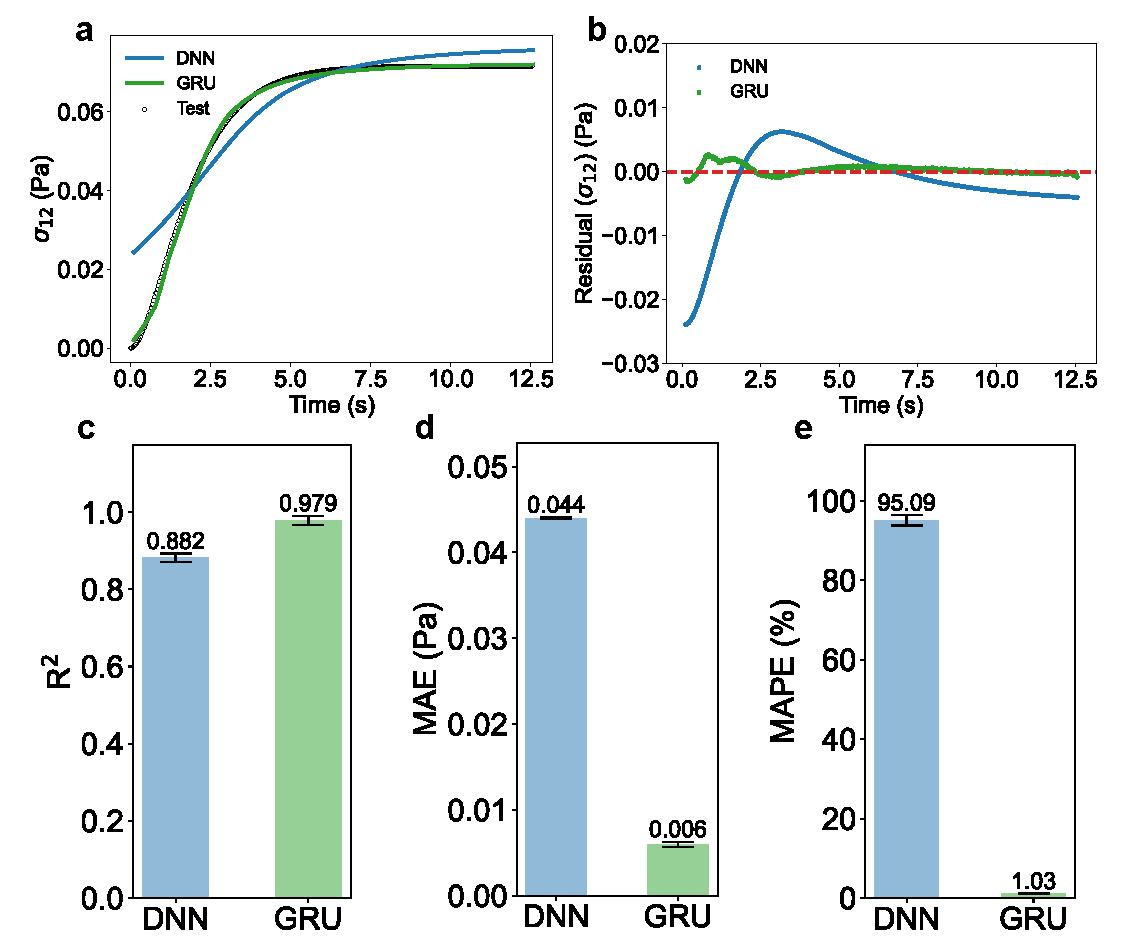
\includegraphics[width=0.8\textwidth]{Fig/doi-edwards-linear.pdf}
  \FigureBicaption{\label{doi-edwards-linear}}{}
\end{figure}

接下来,本节对两种算法在测试集上的预测性能指标进行了详细计算,并绘制了相应的指标对比图,如图\ref{doi-edwards-linear-metrics}所示。从图\ref{doi-edwards-linear-metrics}(a)中可以看出,GRU算法的 R$^2$值达到了0.979,这一结果充分证明了GRU在预测任务中的卓越表现。相比之下,DNN算法的 R$^2$值仅为0.882,明显低于GRU,这表明在 R$^2$指标的评估中,GRU的表现更为出色。进一步观察图\ref{doi-edwards-linear-metrics}(b-c),可以发现GRU预测结果的平均绝对误差(MAE)值为0.006,而DNN的MAE值则高达0.044。这意味着GRU在绝对误差方面的表现仅为DNN的七分之一,优势极为显著。此外,GRU预测结果的平均绝对百分比误差(MAPE)值为1.03,而DNN的MAPE值则为95.09。这些定量数据充分说明了GRU的预测结果误差远小于DNN,从而证明了GRU在该任务上的预测泛化能力更强。
至于训练时间的对比,与上一节中交变协议预测交变协议的情况一致,具体可参考图\ref{doi-edwards-sin-metric}(d)所示。
\begin{figure}[htbp]
  \centering
  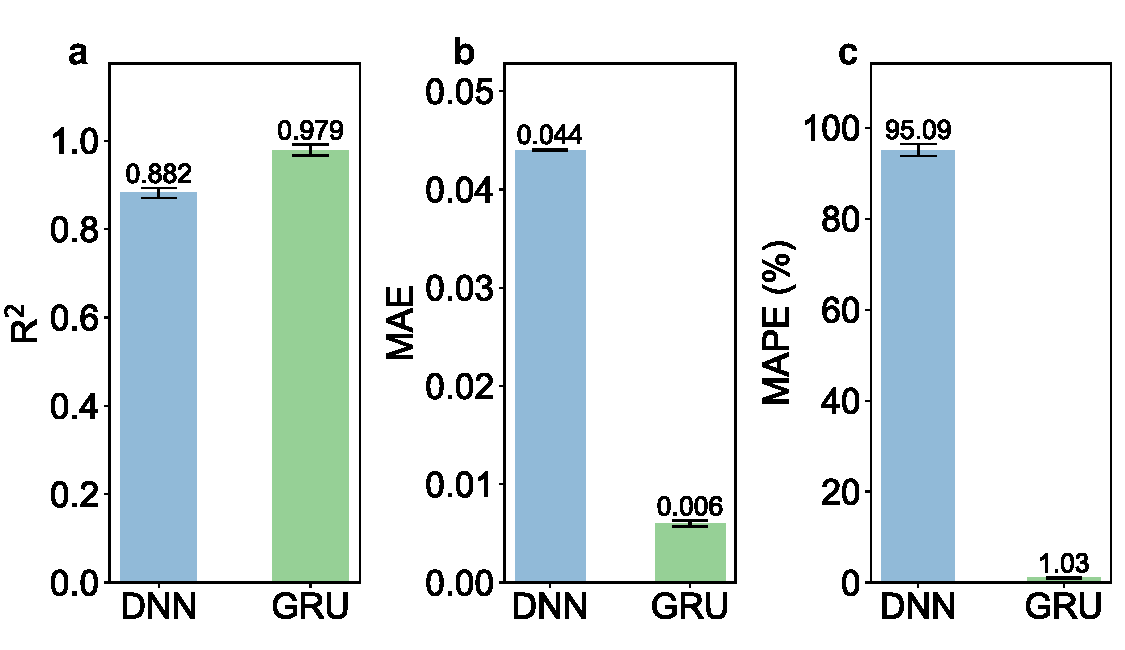
\includegraphics[width=0.8\textwidth]{Fig/doi-edwards-linear-metrics.pdf}
  \FigureBicaption{\label{doi-edwards-linear-metrics}}{}
\end{figure}
从整体分析数据来看,当训练数据与测试数据涉及不同类型的应变变化过程时,GRU算法在学习Doi-Edwards模型数据的内在特性方面有显著优势。这主要归因于GRU算法能够高效地从交变应变数据中提取关键的时间依赖特征,并将其成功应用于线性应变的预测之中。

\subsubsection{不同时间步的预测效果对比}
为了探究在Doi-Edwards模型上GRU算法的最佳时间步,本节研究了不同时间步下训练的模型在测试集上的预测效果,如图\ref{doi-edwards-timesteps-metrics}所示。由图可见,预测模型R$^2$值在时间步小于40时随着时间步的增加而增加,在时间步大于40后反而略有下降。MAE值和MAPE值在时间步小于40时随时间步的增加而减少,时间步为40的值只有不到时间步为20的值的十分之一,显著下降,而时间步大于40后,MAE值和MAPE值则趋于稳定。这说明对于本项任务,时间步为40左右时,恰好可以开始获得不错的预测效果,而从训练成本来看,训练时间是随着时间步设置增加而单调增的,所以综合看来,时间步为40左右时,性价比最高。
\begin{figure}[htbp]
  \centering
  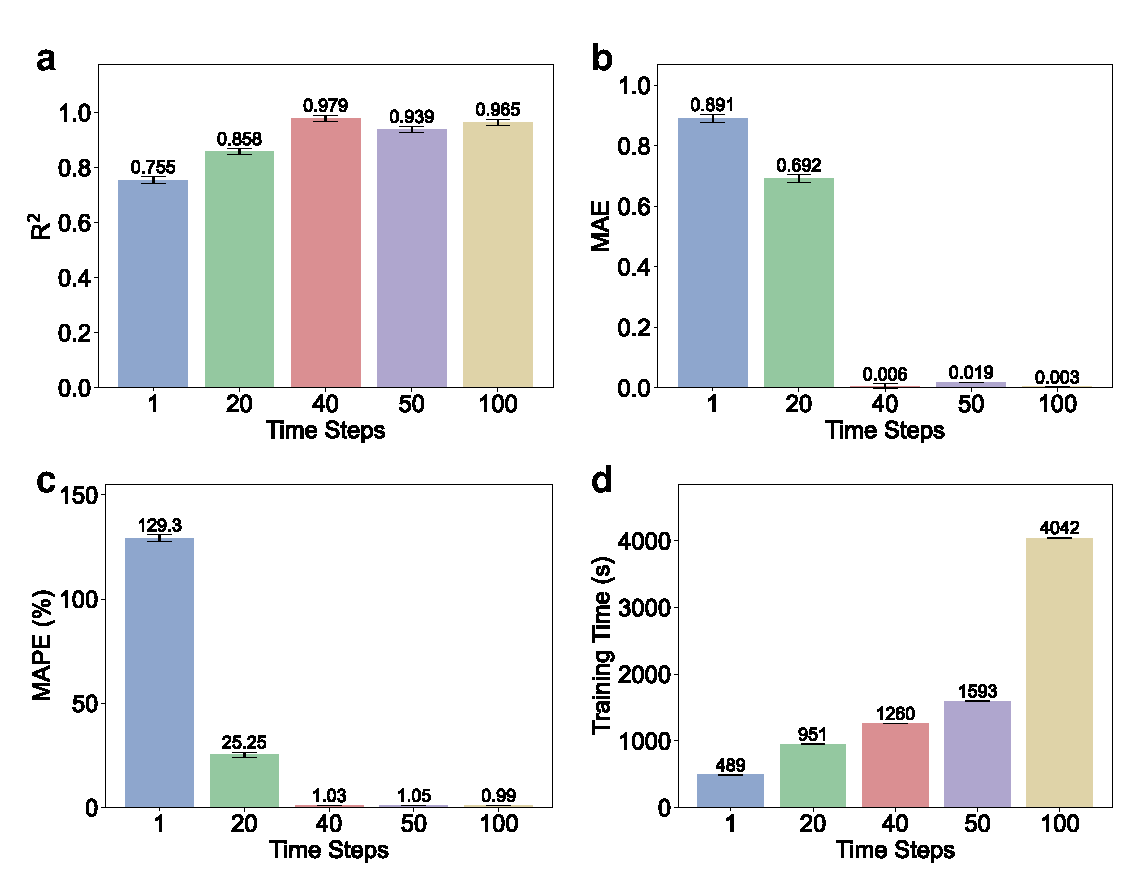
\includegraphics[width=0.8\textwidth]{Fig/doi-edwards-timesteps-metrics.pdf}
  \FigureBicaption{\label{doi-edwards-timesteps-metrics}}{}
\end{figure}
% Giesekus模型建模
\subsection{Giesekus模型建模}
\subsubsection{数值模拟数据}
本节通过Python的微分方程求解库来模拟Giesekus模型,模拟结果如图\ref{giesekus_moni}。

图\ref{giesekus_moni}展示了部分模拟数据,主要展示不同应变振幅下,本构关系从线性本构到非线性的转变。图\ref{giesekus_moni}(a)展示了不同交变应变协议的应力-应变率Lissajous曲线,Protocol 1为小振幅振荡剪切(SAOS)的模拟曲线,呈现椭圆状的滞后环,随着振幅增加,Protocol 2和 Protocol 3呈现非线性特征的扭曲和不对称,这是大振幅振荡剪切(LAOS)的拟合曲线。图\ref{giesekus_moni}(b)展示了不同交变应变协议的第一法向应力差(N$_1$)-应变率Lissajous曲线,随着振幅增加呈现不对称扭曲,曲线形状符合Giesekus模型假设\cite{lennonScientificMachineLearning2023a}。
\begin{figure}[htbp]
  \centering
  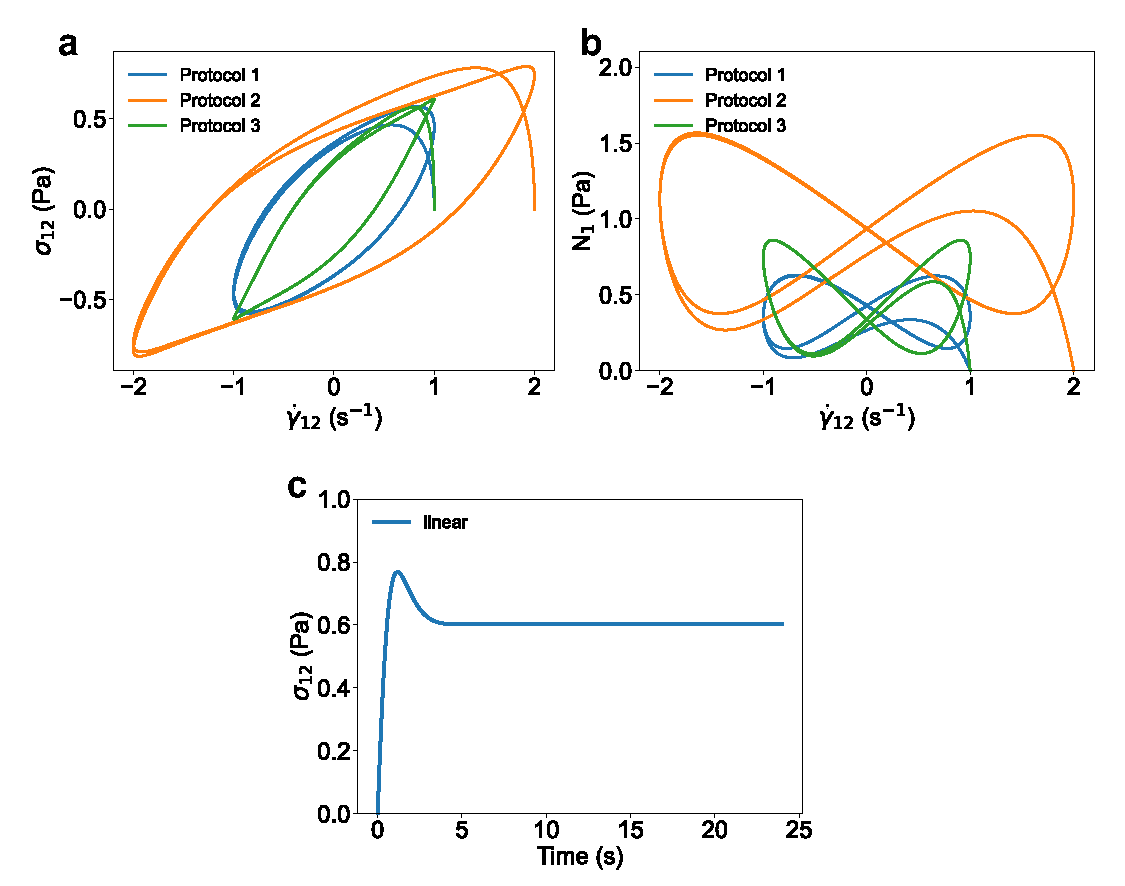
\includegraphics[width=0.8\textwidth]{Fig/giesekus-moni.pdf}
  \FigureBicaption{\label{giesekus_moni}}{}
\end{figure}
图\ref{giesekus_moni}(c)为线性应变协议下的应力-时间曲线,曲线先随着应变加载攀升,存在明显峰值后回落,后趋于稳定。这可能是因为在屈服点之前,材料主要表现出弹性行为,应力随着应变的增加而线性增长。当应力达到峰值时,材料开始发生塑性变形,内部结构发生不可逆的变化,峰值之后,材料的内部结构开始重新组织,形成新的平衡状态,这种重组过程通常伴随着应力的下降与重新平衡。综上,线性协议的曲线符合Giesekus模型对于大剪切应变下材料应力响应的假设,可以用于后续实验。

\subsubsection{交变协议预测交变协议效果验证}
为了评估 GRU 算法在 Giesekus 模型本构方程数据预测中的有效性,本节采用交变应变协议生成的数据作为训练集与测试集,分别运用 GRU 和 DNN 进行模型训练,并在测试集上开展验证工作,测试结果如图 \ref{giesekus_sin}、图 \ref{giesekus-sin-metrics} 所示。

图 \ref{giesekus_sin}(a-c)分别为两种算法构建的预测模型所预测的剪切应力($\sigma_{12}$)的 Lissajous 曲线、时间-应力曲线以及残差图,(d- f)则对应预测的第一法向应力差(N$_{1}$)的Lissajous曲线、时间- 应力曲线与残差图。

从图a和图b可以观察到,GRU算法预测的$\sigma_{12}$值与真实值高度接近,曲线拟合效果理想,而DNN算法在部分区域的预测值存在较大偏差。图 c 的残差图进一步显示,GRU算法预测值与真实值的残差紧密围绕 0 刻度线,呈无序离散分布;相比之下,DNN算法预测值与真实值的残差呈现出明显的曲线规律及周期性特征,且与0刻度线的偏离程度较大,残差分布区间显著宽于GRU部分。残差图的结果有力地表明,GRU成功地学习到了训练数据中的各类特征及复杂的非线性关系,不存在明显的周期性规律,整体残差较小;而DNN存在未能充分学习特征的问题,拟合效果欠佳,未能精准捕捉训练数据的特征。

对于图d、图e和图f所展示的N$_{1}$预测效果,其与$\sigma_{12}$的结果呈现出相似性,即GRU的预测性能优于DNN。进一步对比GRU预测的N$_{1}$值和 $\sigma_{12}$值,发现$\sigma_{12}$值的预测效果更为优异,这可能归因于 $\sigma_{12}$与输入的剪切速率特征 $\dot{\gamma_{12}}$ 之间的函数关系相对简单,且更契合时间叠加原理,从而使得GRU能够更有效地捕捉其时间依赖性及内在联系。这部分的模型结果与Doi-Edwards模型结果类似,对于第一法向应力差(N$_1$),目前的GRU模型存在进一步改进的空间。
\begin{figure}[htbp]
  \centering
  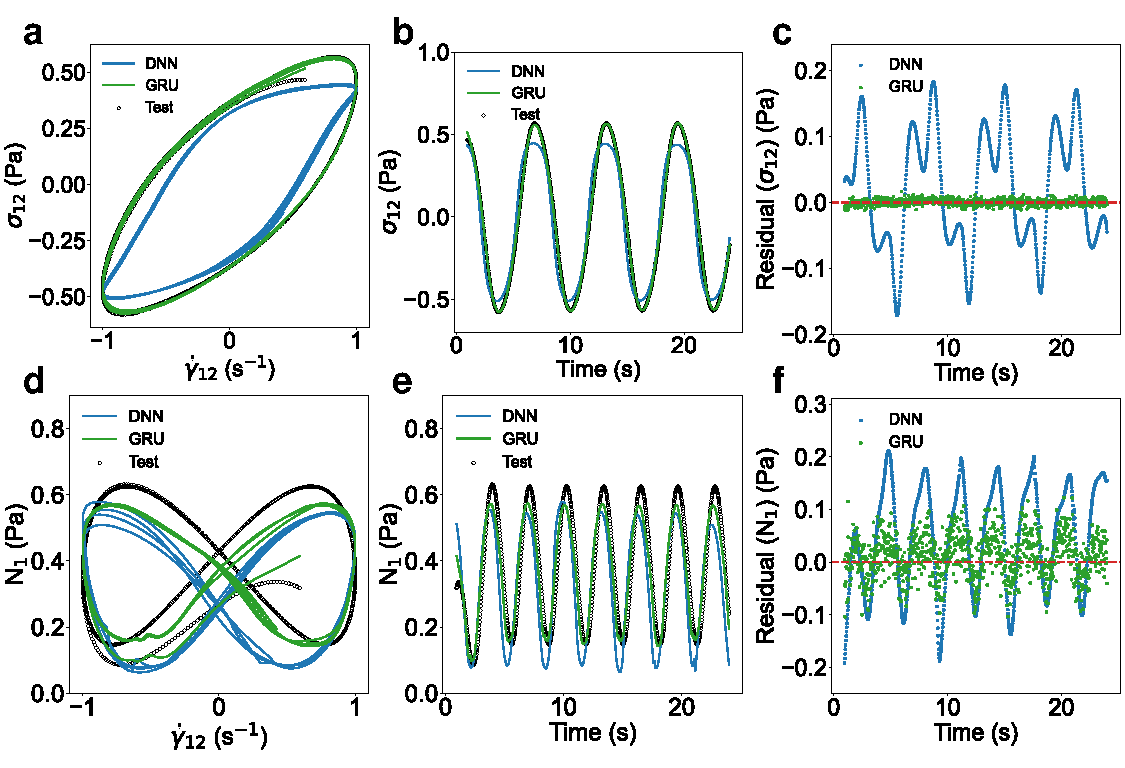
\includegraphics[width=0.8\textwidth]{Fig/giesekus_sin.pdf}
  \FigureBicaption{\label{giesekus_sin}}{}
\end{figure}
在本节中,进一步对两种算法在 $\sigma_{12}$ 和 N$_{1}$ 上的预测效果进行了定量分析,相关指标如图 \ref{giesekus-sin-metrics} 所示。
在 R$^2$指标方面,GRU 在 $\sigma_{12}$ 和 N$_{1}$ 的预测中均优于 DNN。此外,对于同一种算法,$\sigma_{12}$ 的 R$^2$ 值高于 N$_{1}$,例如GRU算法下$\sigma_{12}$的R$^2$值达到0.981,但是对应的N$_{1}$ 的 R$^2$ 值仅达到0.857。
在MAE指标方面,DNN的$\sigma_{12}$和N$_{1}$的MAE值分别为0.079和0.197,均显著高于GRU的0.004和0.051。而在$\sigma_{12}$上,GRU的MAE值为DNN的约二十分之一,对应地,在N$_1$上,GRU的MAE值为DNN的约四分之一。这说明GRU相比DNN的算法领先在$\sigma_{12}$上更为显著。
MAPE值的结果表明相同的结论,DNN预测结果的$\sigma_{12}$和N$_1$分别为112.5\% 和76.81\%,预测结果较差,而GRU的结果为2.68\% 和 15.44\%,预测效果显著优于DNN,且GRU相比DNN在$\sigma_{12}$的优化效果优于N$_1$,这与MAE的结论一致。
最后,从图 \ref{giesekus_sin}(d)可以看出,GRU在此项任务上的训练时间为1156 s,是DNN训练时间的5倍左右,符合其高计算成本的预期。
\begin{figure}[htbp]
  \centering
  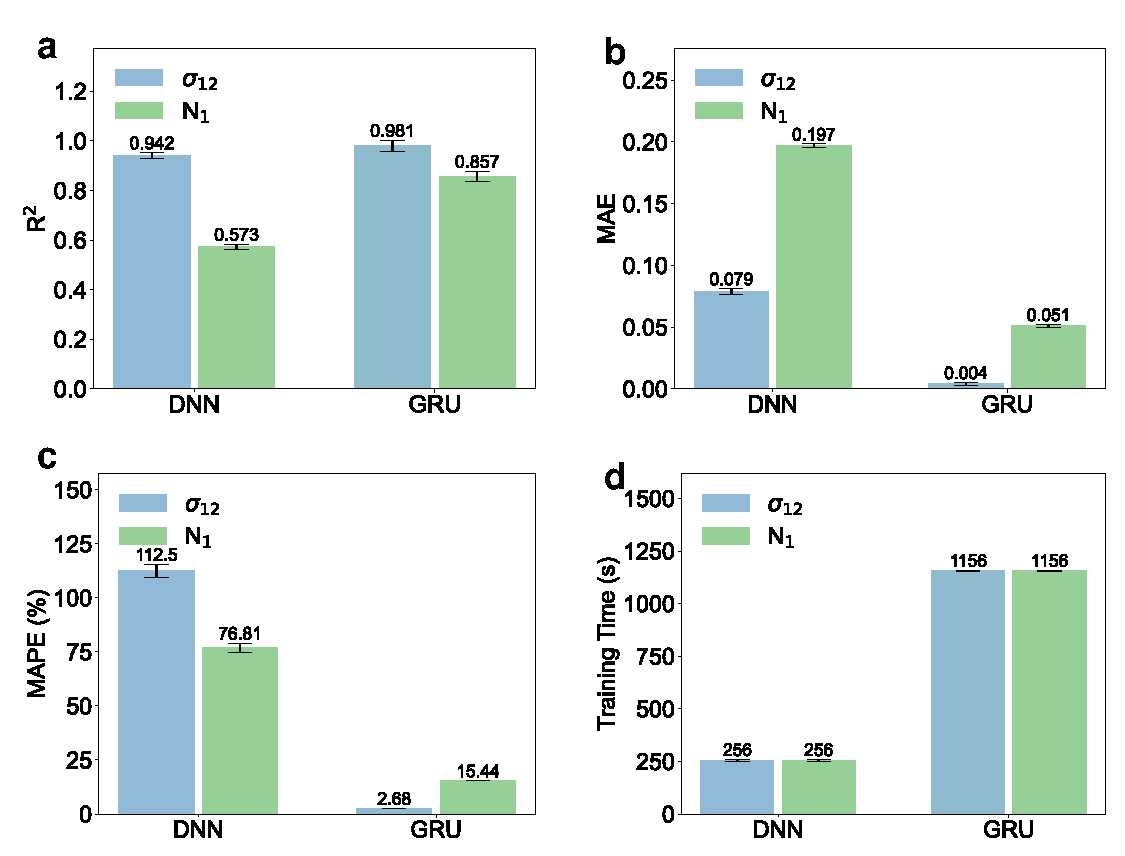
\includegraphics[width=0.8\textwidth]{Fig/giesekus-sin-metrics.pdf}
  \FigureBicaption{\label{giesekus-sin-metrics}}{}
\end{figure}
根据综合分析结果,当训练数据和测试数据均为交变应变时,GRU算法相比DNN能够更好地学习到Giesekus模型数据的内在特征。本节中,我们使用了SAOS和LAOS结合的训练数据,以探究模型对非线性黏弹性的学习能力。结果显示,GRU算法很好地完成了任务,成功捕捉了Giesekus模型模拟数据中的复杂非线性关系。综合来看,GRU算法在处理Giesekus模型的非线性黏弹性数据时表现出了显著的优越性,为后续研究提供了新的视角。

% Giesekus模型交变预测线性协议效果验证
\subsubsection{交变协议预测线性协议效果验证}
为了检验GRU算法在不同形式的应变历史下对Giesekus模型的泛化预测能力,本节采用交变应变协议生成的数据作为训练集,线性应变协议生成的数据作为测试集。分别使用GRU和DNN进行模型训练,并在测试集上进行验证,验证结果如图 \ref{giesekus-linear} 和图 \ref{giesekus-linear-metrics} 所示。

图\ref{giesekus-linear}(a)为两种不同算法预测模型在测试集上的真实值-预测值曲线,图中可以看到GRU算法的预测值的曲线与真实值曲线接近,仅在1-2 s之间存在小部分突出偏差,而DNN算法的预测值曲线完全没有拟合到曲线特征。图\ref{giesekus-linear}(b)展示了两种算法在测试集上的残差图。从图中可以明显看出,DNN算法的预测值与真实值之间的残差整体呈现出较为清晰的曲线趋势,存在明显的峰值。图中结果表明DNN完全没有捕捉到训练数据中的关键特征,导致其在测试集上的表现很差。与之形成鲜明对比的是,GRU 算法的残差图呈现出无序分布的特征,残差点均匀地分布贴近在 0 刻度线两侧。这一现象表明,GRU 能够更有效地学习数据中的关键特征,从而实现更小的预测偏差。结合真实值与预测值的曲线分析以及残差图的观察,可以分析出GRU在此项任务的预测性能优于DNN。
\begin{figure}[htbp]
  \centering
  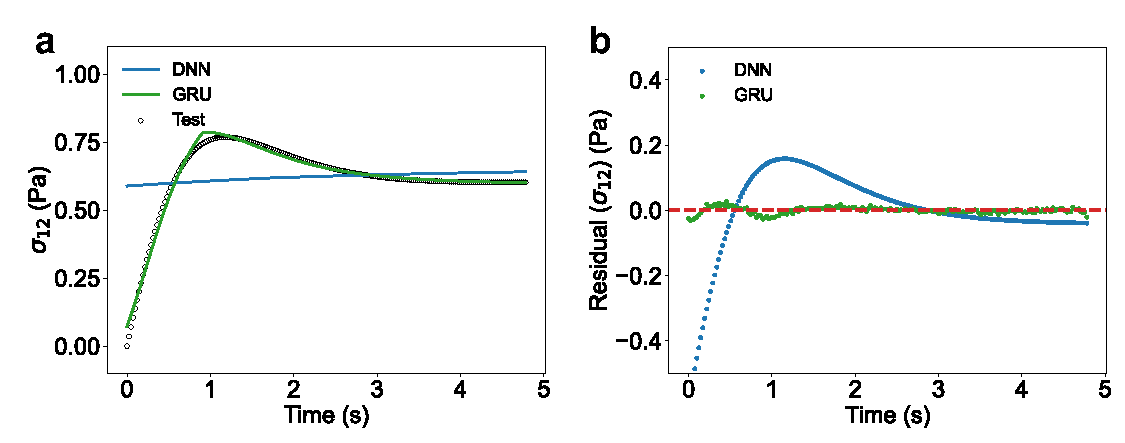
\includegraphics[width=0.8\textwidth]{Fig/giesekus-linear.pdf}
  \FigureBicaption{\label{giesekus-linear}}{}
\end{figure}

具体如图\ref{giesekus-linear-metrics} 所示。从图\ref{giesekus-linear-metrics}(a)可以清晰地观察到,GRU 算法的 R$^2$值高达 0.989,这一结果有力地表明了 GRU 在预测任务中的出色表现。与之形成鲜明对比的是,DNN算法的R$^2$值小于 0,这表明 DNN 并未有效学习到相关特征。进一步分析图\ref{giesekus-linear-metrics}(b-c),可以发现 GRU 预测结果的平均绝对误差(MAE)值为 0.008,而 DNN的 MAE 值则高达 0.083。这表明GRU 在绝对误差方面的表现仅为DNN的十分之一,优势极为明显。此外,GRU 预测结果的平均绝对百分比误差(MAPE)值为2.62\%,而DNN 的 MAPE 值则为 29.41\%。这些定量数据充分证明了 GRU 的预测结果误差小于 DNN,从而进一步证实了 GRU 在该任务上的预测泛化能力更强。
在两种算法的训练时间对比方面,与上一节中交变协议预测交变协议的情况相同,具体可参考图 \ref{giesekus-sin-metrics}(d)所示。
\begin{figure}[htbp]
  \centering
  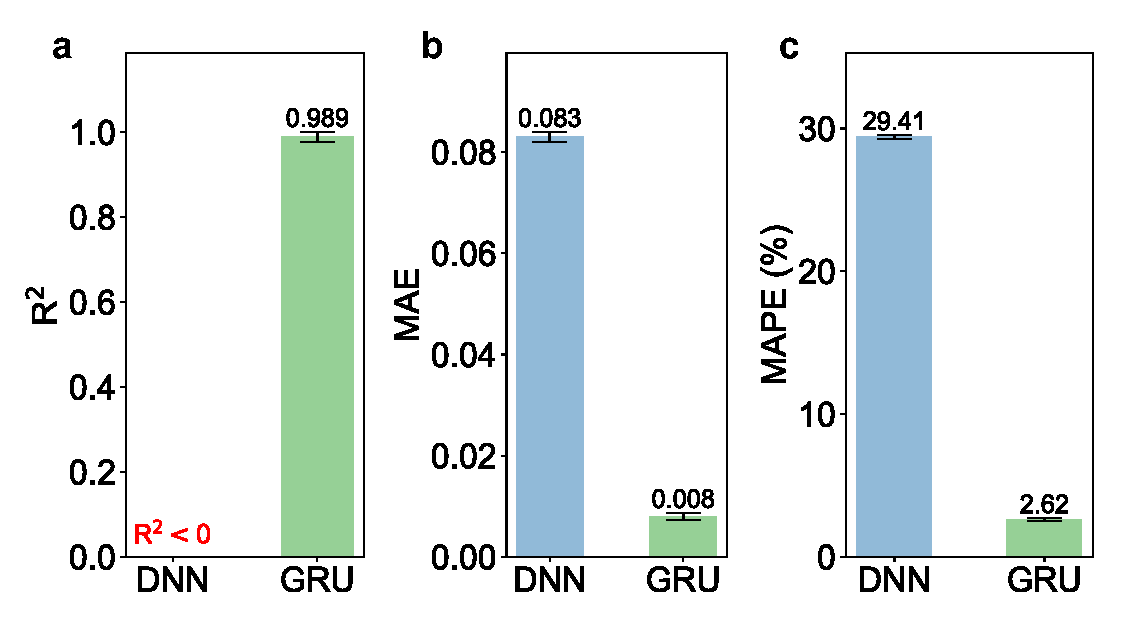
\includegraphics[width=0.8\textwidth]{Fig/giesekus-linear-metrics.pdf}
  \FigureBicaption{\label{giesekus-linear-metrics}}{}
\end{figure}
\subsubsection{不同时间步的预测效果对比}
为了探究在Giesekus模型上GRU算法的最佳时间步,本节研究了不同时间步下训练的模型在测试集上的预测效果,如图\ref{giesekus-timesteps-metrics}所示。由图可见,预测模型R$^2$值在时间步小于40时为0.7左右,当时间步为40时为0.969,时间步进一步增加,R$^2$开始下降。MAE值在时间步为40相比20时从0.306调跃减少至0.008,进一步增加时间步,MAE值不再显著改变,直到时间步为100,MAE值回升至0.156,显现过拟合趋势。MAPE值变化趋势与MAE值类似,在时间步为40左右跳跃减少,随后直到100步开始回升。从训练时间来看,随着时间步增加,训练时间单调增加,这一点与预期一致。
\begin{figure}[htbp]
  \centering
  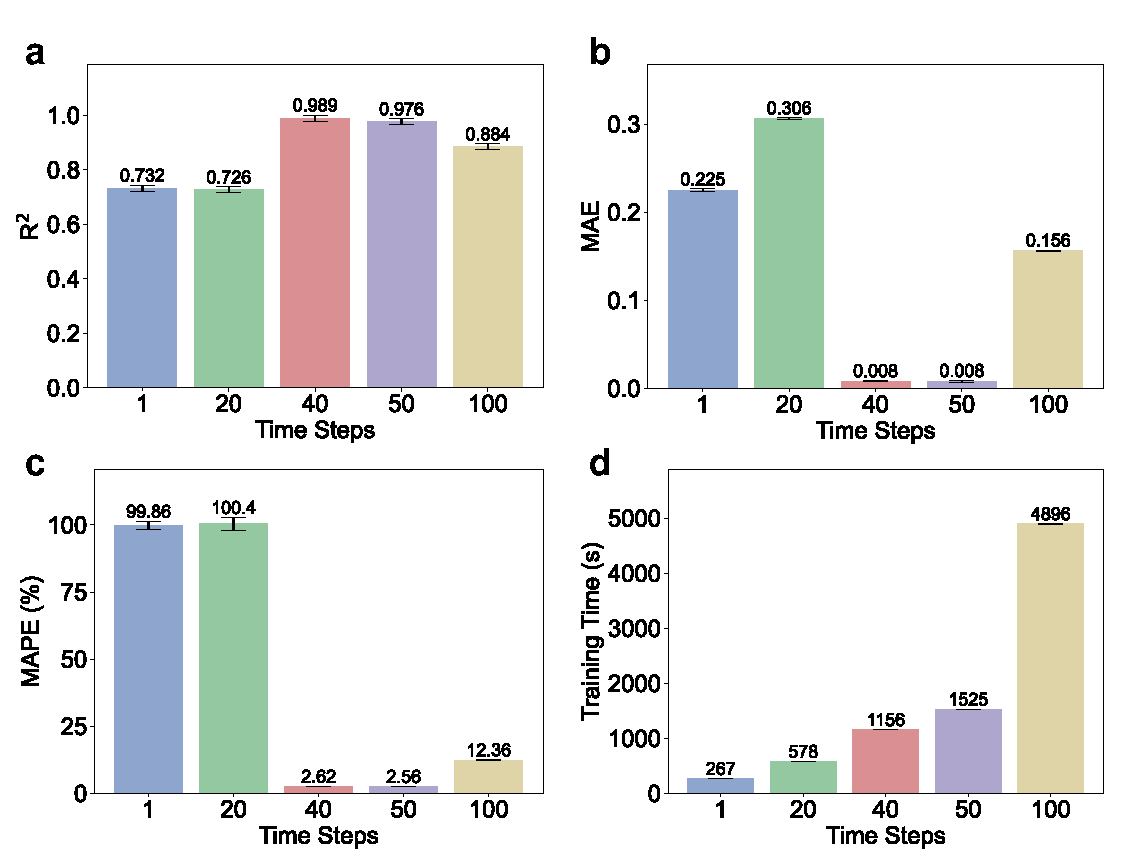
\includegraphics[width=0.8\textwidth]{Fig/giesekus-timesteps-metrics.pdf}
  \FigureBicaption{\label{giesekus-timesteps-metrics}}{}
\end{figure}
\section{本章小结}
本章运用了GRU(门控循环单元)算法对数值模拟的 Herschel-Bulkley 模型、Maxwell 模型、Doi-Edwards 模型以及 Giesekus 模型所产生的模拟数据展开深度学习建模工作。

研究结果揭示出,GRU 作为一种循环神经网络,依托其独特的门控单元机制,能够精准地捕捉黏弹性材料流变学模拟数据所蕴含的时间依赖性以及复杂非线性特征。在处理 Herschel-Bulkley 模型这类非时间序列数据时,GRU 模型的预测效果相较于 DNN(深度神经网络)模型略胜一筹。究其原因,在于 GRU 的门控单元机制引入了更多的参数,从而赋予了其更佳的泛化性能。对于经典的简单 Maxwell模型,鉴于其属于典型的时间序列数据,GRU 对其进行建模预测的效果全面超越DNN,各项评估指标均展现出显著优势。这一现象主要得益于 GRU 的门控循环单元机制,该机制能够有效地控制材料历史记忆的流动与记录过程。当面对更为复杂Doi-Edwards 模型时,GRU的建模预测效果依旧优于 DNN。进一步分析发现,在相同的建模任务中,GRU 在剪切应力$\sigma_{12}$的预测效果上强于第一法向应力差N$_1$,这主要是由于输入特征为剪切速率,而剪切速率与剪切应力之间存在着更为直接的关联。在Giesekus 模型的研究中,本章模拟了小振幅振荡剪切(SAOS)以及大振幅振荡剪切(LAOS)这两种不同的工况。实验结果表明,GRU 的建模效果优于 DNN,这有力地说明 GRU 所捕捉的时间依赖性,不仅仅局限于基于玻尔兹曼叠加原理的线性黏弹性的时间特性,还能够涵盖更为复杂的非线性关系,而Giesekus模型下GRU对第一法向应力差N$_1$的预测效果也比$\sigma_{12}$差。

在本章设计的实验中,我们探讨了两类预测任务:首先,利用交变应变变化的训练数据,预测相应的测试数据;其次,使用交变应变变化实验的训练数据,预测线性应变变化的测试数据。在针对不同本构模型的这两类实验中,GRU(门控循环单元)模型的表现均优于DNN(深度神经网络)。这一现象充分表明,GRU具备更强的泛化能力,能够有效地预测更为一般化的本构关系,而不仅仅是进行简单的函数逼近。GRU通过引入门控机制,能够有效捕捉序列数据中的长期依赖关系,从而在处理复杂的本构模型时展现出更优的性能。相比之下,DNN虽然在非时序本构模型中表现出色,但在处理具有复杂时序特征的本构模型时,其性能会受到限制。因此,选择GRU模型进行本构关系的预测,能够更好地适应数据的复杂性和多样性,提升预测的准确性和可靠性,但是本章的实验结果同样表明,GRU模型由于其架构特征,比普通DNN的训练时间高很多,且训练时消耗更多的计算机资源(计算机内存、GPU显存等)。可以预见的是,在超大型数据集上,GRU的训练成本会远远大于DNN。

综上所述,本章的研究工作充分验证了GRU模型在流变学数据建模中的优异效果。该模型不仅能够准确捕捉黏弹性材料的时间依赖性,从而高效刻画非线性、时变的物理过程,展现出良好的关联适配性,而且在理论上突破了传统数据拟合方法的局限,在模拟数据实践中表现出卓越的泛化能力和预测稳定性,为进一步开展真实实验中的流变学数据研究提供了坚实依据。总的来说,本章的研究为深度学习在流变学本构建模领域的应用开辟了全新的思路,即可以从模型升级的角度去优化本构建模的过程。











